\documentclass[11pt]{article}
\usepackage[margin=1in]{geometry}
\usepackage{amsmath}
\usepackage{graphicx}
\usepackage{tikz-cd}
\usepackage{multicol}
\usepackage{xcolor}
\usepackage{tabularx}
\usepackage{enumitem}
\usepackage{subcaption}
\usepackage{float}
\usepackage{svg}

\setlength{\parindent}{0pt}
\setlength{\parskip}{1\baselineskip}
\numberwithin{figure}{section}
\setcounter{tocdepth}{2}

\begin{document}
\begin{titlepage}
  \newgeometry{margin=1in}
  \thispagestyle{empty}
  \centering
  
\includegraphics[width=4.2cm]{images/immagine_2026-03-10_163746246.png}

  \vspace*{1.3cm}
  {\fontsize{28}{30}\selectfont\textcolor[rgb]{0.0,0.28,0.43}{\textsc{Università degli Studi dell'Aquila}}\par}

  \vspace*{1.2cm}
  {\fontsize{21}{23}\selectfont\textsc{Facoltà di Informatica}\par}

  \vspace*{1.1cm}
  {\fontsize{20}{22}\selectfont\textsc{Applicazioni per dispositivi mobili}\par}

  \vspace*{1.2cm}
  {\fontsize{24}{26}\selectfont\bfseries\itshape JAMB\par}

  \vspace*{0.45cm}
  \includesvg[width=3.2cm]{images/Group5}

  \vfill
  \noindent
  \begin{tabularx}{\textwidth}{@{}l X r@{}}
    \begin{minipage}[t]{0.42\textwidth}
      \raggedright
      Prof.\\[0.8em]
      Bucchiarone Antonio
    \end{minipage}
    &
    \begin{minipage}[t]{0.16\textwidth}
    \end{minipage}
    &
    \begin{minipage}[t]{0.50\textwidth}
      \raggedleft
      Studente\\[0.8em]
      Matteo Cardarelli 292215\\[0.6em]
    \end{minipage}
  \end{tabularx}
\end{titlepage}
\restoregeometry

\tableofcontents

\newpage
\section*{Glossario dei termini scout}
\addcontentsline{toc}{section}{Glossario dei termini scout}

Il dominio applicativo adotta un lessico proprio del metodo scout. I termini
ricorrenti nel documento sono raccolti qui.

\begin{description}\setlength{\itemsep}{0.4em}

\item[AGESCI] Associazione Guide e Scouts Cattolici Italiani, l'associazione
di riferimento del progetto.

\item[Gruppo] L'unità organizzativa territoriale di base, che riunisce tutte
le branche presenti in una stessa località.

\item[Branca] La suddivisione per fascia d'età. Lupetti e Coccinelle (L/C)
dagli otto agli undici anni, Esploratori e Guide (E/G) dai dodici ai sedici,
Rover e Scolte (R/S) dai diciassette ai ventuno.

\item[Unità] Il gruppo di ragazzi di una singola branca, con il proprio staff
di capi. L'unità della branca E/G prende il nome di Reparto.

\item[Squadriglia] Il gruppo permanente di sei-otto ragazzi in cui si articola
il Reparto, guidato da un Capo Squadriglia affiancato da un Vice.

\item[Alta Squadriglia] L'insieme dei ragazzi più grandi del Reparto,
provenienti da squadriglie diverse, che svolgono attività proprie.

\item[Consiglio Capi] L'organo del Reparto formato dai Capi Squadriglia e
dallo staff, dove si prendono le decisioni sulla vita dell'unità.

\item[Comunità Capi (Co.Ca.)] L'assemblea di tutti i capi adulti del Gruppo,
di ogni branca, responsabile delle scelte educative complessive.

\item[Progetto Educativo di Gruppo (PEG)] Il documento pluriennale con cui la
Comunità Capi fissa gli obiettivi educativi dell'intero Gruppo.

\item[Programma d'Unità] Il documento annuale con cui lo staff di una singola
unità declina gli obiettivi del PEG in traguardi verificabili per la propria
branca. È il documento gestito dall'applicazione.

\item[Sentiero] Il percorso di crescita personale del ragazzo in branca E/G,
articolato nelle tappe della Scoperta, della Competenza e della
Responsabilità, ciascuna con i propri impegni.

\item[Specialità] Il riconoscimento di una competenza pratica acquisita dal
ragazzo, ottenuto superando le prove previste.

\item[Brevetto] Il riconoscimento di livello superiore alla specialità, che
attesta la padronanza di un'area di competenza e presuppone il conseguimento
di più specialità collegate.

\item[Impresa] L'attività ideata, progettata e realizzata autonomamente da una
squadriglia, dalla proposta iniziale alla verifica finale.

\item[Uscita] L'attività di una o due giornate fuori sede, tipicamente nel
fine settimana.

\item[Campo] L'attività residenziale di più giorni, generalmente estiva.

\item[Route] Il campo itinerante, caratteristico della branca R/S, percorso a
piedi con cambio di località ogni giorno.

\item[Punto della Strada] Il momento di verifica personale del percorso di
crescita, proprio della branca R/S.

\item[Assistente Ecclesiastico (A.E.)] Il sacerdote che affianca la Comunità
Capi nell'accompagnamento spirituale.

\item[Censimento] L'iscrizione annuale del socio all'associazione, condizione
necessaria per la copertura assicurativa e la partecipazione alle attività.

\item[Capo Gruppo] Il responsabile dell'intero Gruppo, unico ruolo con
competenza su tutte le unità.

\item[Capo Unità] Il responsabile di una singola unità.

\item[Aiuto Capo] Il capo che affianca il Capo Unità nella conduzione
dell'unità e nel lavoro diretto con i ragazzi.

\end{description}

\newpage

\section{Introduzione}
\subsection{Contesto del progetto e motivazioni}
Lo scautismo è uno dei movimenti educativi più grandi al mondo, con centinaia di migliaia di iscritti solo in Italia. Il progetto nasce dal fatto che l'organizzazione quotidiana di un gruppo scout richiede una gestione della logistica veramente dispersiva e complessa, quasi sempre basata su metodi cartacei.

Ho scelto di lavorare su questo progetto per risolvere criticità organizzative, che compromettono lo scopo educativo perseguito dai Soci Adulti Educanti. "\textbf{\textit{Jamb}}" punta a ridurre il carico burocratico, per lasciare più spazio allo scopo educativo, ed aiutare nella gestione della sicurezza e della responsabilità legale. Tutto ciò senza dimenticare i ragazzi, fulcro del lavoro dei Soci Adulti, a cui saranno dedicate sezioni apposite per: tracciare il proprio sentiero/percorso; aiutare anche loro a gestire i propri progetti.


\subsection{Scopo generale dell'applicazione}
Lo scopo dell'applicazione è creare un ecosistema digitale "all-in-one" per lo scautismo, unendo l'organizzazione logistica al percorso educativo. Per i capi, l'obiettivo è semplificare la burocrazia: l'app deve sostituire numerosi registri cartacei in un solo posto. Per i ragazzi, invece, lo scopo è renderli protagonisti, fornendo loro degli strumenti per avere sempre sott'occhio il proprio percorso e il proprio sviluppo personale, inoltre l'app li aiuta nella gestione delle attività che saranno organizzate con altri ragazzi.

\subsection{A chi è destinata, quale problema risolve}
L'app è progettata per supportare l'organizzazione logistica e il percorso educativo all'interno dello scautismo e si rivolge a due categorie principali di utenti:
\begin{itemize}[topsep=0.5pt]
  \item \textbf{Capi (educatori):} è destinata ai soci adulti che amministrano il gruppo e le singole unità. L'applicazione facilita la visualizzazione, l'organizzazione e la gestione delle presenze, degli eventi e delle scadenze legali/mediche.
  \item \textbf{Ragazzi (giovani dagli 11 ai 21 anni):} è destinata ai membri delle varie unità (E/G, R/S) che vivono in prima persona l'esperienza scout. Lo scopo dell'app per questa categoria di utenti è offrire loro un punto di accesso semplice per tracciare il proprio percorso di crescita e gestire i progetti delle pattuglie.
\end{itemize}

Il bisogno a cui l'app risponde è l'esigenza di uno strumento unico, integrato e funzionante anche offline per la gestione delle attività scout. Nello specifico \textit{\textbf{Jamb}} nasce per alleggerire il carico organizzativo e burocratico dei capi, eliminando la dispersione causata dai vari e sparsi fogli Excel, chat e moduli cartacei, ottimizzando i tempi di pianificazione.

\newpage

\section{Scelta e Analisi del Dominio}
\subsection{Descrizione del dominio applicativo scelto}
Il dominio applicativo scelto è la \textbf{Gestione Organizzativa ed Educativa dello Scautismo}. Si tratta di un ambito operativo complesso e fortemente stratificato, che unisce le necessità amministrative di un'organizzazione associativa con le dinamiche pedagogiche e logistiche. Attualmente questo settore è caratterizzato da una forte frammentazione degli strumenti e da una digitalizzazione, dove presente, non centralizzata, che rallenta fortemente i processi organizzativi ed amministrativi. L'introduzione di una soluzione digitale, progettata per operare anche in assenza di rete, consentirebbe di velocizzare notevolmente la burocrazia e automatizzare la raccolta di dati sul campo.

\subsection{Motivazione della scelta}
La scelta di questo dominio applicativo è fortemente radicata in un'esperienza diretta e personale all'interno del contesto associativo. Il recente ingresso da parte mia nella Comunità Capi (Co.Ca.) mi ha permesso di percepire il profondo divario tra la missione pedagogica dello scautismo e la complessa realtà organizzativa. Ho avvertito l'esigenza di riunire in un unico posto la burocrazia frammentata. Pertanto, la progettazione di \textit{\textbf{Jamb}} nasce dalla volontà di risolvere una criticità vissuta in prima persona.

\subsection{Analisi dei problemi o delle opportunità del dominio}
L'analisi del dominio evidenzia svariate criticità, a partire dalla gestione di una mole massiccia di dati e documenti estremamente sensibili, come schede sanitarie e liberatorie per la privacy dei minori, la cui archiviazione malgestita espone a gravi rischi legali. A questo si aggiunge la difficoltà strutturale nell'affiancarsi a sistemi gestionali associativi già esistenti, spesso obsoleti, poco usabili via mobile e completamente privi di uno standard moderno. Il panorama attuale è caratterizzato da uno scarso stato dell'arte e da un mercato sostanzialmente privo di competitor diretti che offrano una soluzione integrata, questo rappresenta una sfida notevole ed ambiziosa data la mole di lavoro necessario per coprire tutte le esigenze del metodo scout. 

Tuttavia, queste criticità generano opportunità uniche. La forte conoscenza del dominio derivata dall'esperienza diretta permette di progettare un'interfaccia creata su misura per le reali abitudini dei capi, garantendo un accesso diretto agli utenti finali durante lo sviluppo. Nonostante si tratti di un'app mai realizzata, l'assenza di uno standard moderno offre il vantaggio competitivo di poter definirne uno nuovo. L'opportunità si può trovare nel trasformare la complessa burocrazia in un sistema fluido e sicuro, capace di funzionare anche in contesti isolati e di fornire ai ragazzi e ai capi uno strumento all'altezza delle sfide educative.

\newpage
\section{Analisi del Progetto}
\subsection{Analisi SWOT}
L'analisi SWOT sintetizza i punti di forza e di debolezza intrinseci al progetto, insieme alle opportunità e alle minacce derivanti dal contesto esterno. Questa valutazione è fondamentale per definire una strategia di sviluppo che massimizzi i vantaggi competitivi e diminuisca i rischi operativi.

\begin{itemize}[topsep=0.5 pt]
  \item \textbf{Punti di Forza (Strengths):}
  Il principale vantaggio consiste nella profonda conoscenza del dominio, che permette di progettare un'esperienza utente modellata sulle reali necessità degli utenti finali, evitando funzionalità superflue. Inoltre molti capi richiedono da tempo una digitalizzazione della burocrazia che occupa spesso buona parte del tempo, che invece vorrebbe essere dedicata alla progettazione di attività. Dal punto di vista tecnico, l'utilizzo di un'architettura \textbf{Offline-First} rappresenta una funzione fondamentale, garantendo l'affidabilità del sistema anche in condizioni ambientali isolate. Inoltre, la scelta di una struttura tecnologica moderna e scalabile (Flutter e Supabase) consente di ottenere alte prestazioni con costi di infrastruttura ridotti, facilitando un eventuale rilascio su larga scala.

  \item \textbf{Punti di Debolezza (Weaknesses):}
  La criticità maggiore è rappresentata dalla mole massiccia di lavoro richiesto per coprire l'intero ambiente scout, essendo un progetto sviluppato da un singolo sviluppatore in tempi accademici, lo \textit{scope} iniziale deve essere necessariamente limitato a un MVP (Minimum Viable Product). Inoltre essendo il progetto di un singolo non si coprono tutte le aree richieste per la progettazione totale del progetto, con il rischio di rilasciare un'app con delle mancanze dovute alla scarsa conoscenza ed esperienza del singolo. Un altro punto di debolezza è lo scarso stato dell'arte: non esistendo standard moderni a cui ispirarsi, ogni modulo deve essere progettato da zero, aumentando il rischio di complessità logica nell'interfaccia. 

  \item \textbf{Opportunità (Opportunities):}
  Il mercato attuale presenta un'assenza quasi totale di competitor diretti che offrano una soluzione integrata e mobile-native, creando un'opportunità di posizionamento come standard moderno per le associazioni scout. La possibilità di accesso diretto ai clienti (i gruppi scout del territorio) permette una validazione rapida dell'app e una raccolta di feedback immediata. L'app si potrebbe estendere anche ad associazioni diverse dall'A.G.E.S.C.I. con non troppo sforzo, aumentando così il bacino di utenza.

  \item \textbf{Minacce (Threats):}
  La minaccia principale è legata alla difficoltà di integrazione con i sistemi già esistenti a livello nazionale, che potrebbero complicare l'adozione ufficiale dell'app. Esiste inoltre il rischio legato alla gestione di dati estremamente sensibili (sanitari e privacy di minori): eventuali errori potrebbero cambiare drasticamente la fiducia degli utenti ed evolversi in rischi legali. Inoltre la resistenza al cambiamento di alcuni utenti legati ai metodi analogici potrebbe rallentare la diffusione dell'applicazione. Il progetto non è fornito di fondi economici a cui attingere, questo potrebbe creare problemi con una diffusione più ampia dell'app, che porterebbe dei costi richiesti dai servizi utilizzati per l'immagazzinamento dei dati.
\end{itemize}

\newpage

\subsection{Analisi degli attori}
L'efficacia di \textbf{\textit{Jamb}} è la capacità di riflettere l'organizzazione scout così come è all'interno dell'A.G.E.S.C.I. Definire chi interagisce con l'applicazione permette di costruire un sistema sicuro, dove l'accesso alle informazioni è regolato dal ruolo ricoperto all'interno del gruppo o della branca. Questa separazione è fondamentale per proteggere la riservatezza dei percorsi educativi, assicurando che ogni utente visualizzi solo ciò che è pertinente al proprio servizio o al proprio sentiero di crescita.

\begin{figure}[h]
  \centering
  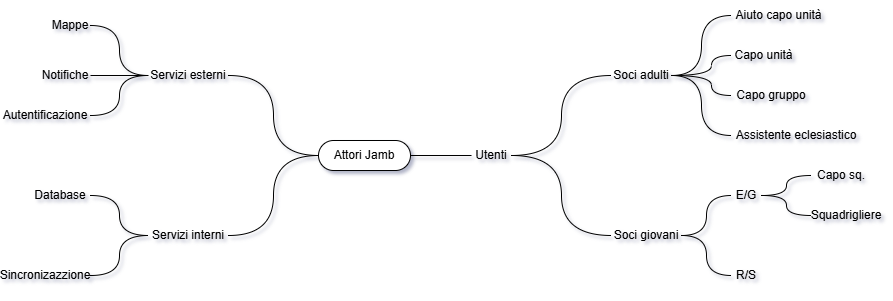
\includegraphics[width=15cm]{images/mindMap.png}
  \caption{Mappa concettuale degli attori del sistema.}
  \label{fig:mindmap}
\end{figure}

La struttura mostrata nella mappa separa le componenti umane del progetto da quelle tecniche necessarie a sostenerle. Il sistema ruota attorno a due categorie principali: i Soci Adulti e i Soci Giovani. Per gli adulti, \textbf{\textit{Jamb}} si focalizza sulla semplificazione burocratica e sulla gestione logistica, fornendo strumenti differenziati per chi opera a stretto contatto con i ragazzi nelle unità e per chi coordina la vita dell'intero gruppo. Sul fronte dei ragazzi, l'attenzione si sposta sul protagonismo e sul tracciamento della propria progressione personale, con permessi che variano per supportare chi ha compiti di responsabilità verso i propri pari.


A supporto di queste figure agiscono i servizi interni ed esterni, che rappresentano il motore tecnico dell'applicazione. I servizi interni, come il database e il sistema di sincronizzazione, garantiscono che i dati siano sempre aggiornati e consultabili anche in zone prive di copertura di rete, condizione comune durante le attività all'aperto. I servizi esterni completano l'ecosistema fornendo le funzionalità necessarie alla vita scout, dalla cartografia per la pianificazione dei percorsi alle notifiche per le comunicazioni urgenti, fino ai sistemi di autenticazione.

\newpage

\section{Obiettivi del Progetto}
\subsection{Obiettivi generali}
\begin{enumerate}
  \item \textbf{Riduzione del carico burocratico}
  Automatizzare la gestione dei registri cartacei, dei censimenti e delle scadenze legali/mediche in un unico punto di accesso digitale.
  \item \textbf{Gestione centralizzata della sicurezza}
  Fornire ai Soci Adulti strumenti immediati per la consultazione dei dati critici (allergie, farmaci, autorizzazioni) anche in assenza di connettività, garantendo la responsabilità legale e assicurativa.
  \item \textbf{Ottimizzazione della logistica di Zona}
  Facilitare il coordinamento tra i Capi Gruppo e il Comitato di Zona per l'organizzazione di eventi complessi (es. San Giorgio, Moduli formativi) attraverso flussi di lavoro strutturati.
  \item \textbf{Monitoraggio del Progetto Educativo di Gruppo (PEG)}
  Offrire dashboard analitiche per valutare l'andamento del PEG e la continuità educativa tra le branche.
  \item \textbf{Tracciamento dell'Iter formativo}
  Gestire lo storico della formazione dei capi (Campi di formazione, nomina a capo) per supportare la crescita della Comunità Capi.
  \item \textbf{Archivio Metodologico Dinamico}
  Centralizzare l'accesso a documenti ufficiali AGESCI, pillole metodologiche e kit per le attività, facilitando la progettazione delle attività.
  \item \textbf{Digitalizzazione della progressione personale}
  Fornire agli E/G e agli R/S strumenti per tracciare il proprio \textit{"sentiero"} o \textit{"strada"}, rendendoli protagonisti consapevoli della propria crescita.
  \item \textbf{Supporto alla metodologia di branca}
  Implementare moduli specifici che riflettano le strutture metodologiche come la gestione delle Imprese per le Squadriglie (E/G) e la pianificazione dei Capitoli per il Clan (R/S).
  \item \textbf{Gamification Educativa}
  Trasformare il monitoraggio della progressione personale in un'esperienza stimolante, incentivando la consapevolezza del proprio percorso senza aggiungere carichi gestionali eccessivi.
  \item \textbf{Operatività in ambienti isolati (Offline-First)}
  Garantire la piena funzionalità dell'app durante l'attività in ambienti isolati, grazie alla sincronizzazione asincrona.
  \item \textbf{Sicurezza e privacy by design}
  Implementare una gestione dei dati basata su Row-Level Security (RLS) e Role-Based Access (RBAC), assicurando che le informazioni sensibili (dati medici, Punto della Strada) siano accessibili solo a chi ne ha il diritto metodologico e legale.
  \item \textbf{Multi-tenancy Associativa}
  Gestire in modo isolato ma comunicante i diversi livelli dell'associazione (Gruppo e Zona), permettendo comunicazioni segmentate e gestione di eventi multi-unità.
\end{enumerate}

\newpage

\subsection{Obiettivi Funzionali}
\subsubsection{Gestione dei livelli per i soci adulti}
Per garantire un'interfaccia pulita e una gestione sicura dei dati, l'architettura di Jamb adotta un modello di permessi "a matrioska". Questo significa che i ruoli di responsabilità superiore ereditano automaticamente e in modo trasparente tutte le funzionalità, le viste e i permessi dei ruoli sottostanti, rispecchiando le dinamiche operative della Comunità Capi (Co.Ca.) e delle Unità. La cascata si struttura così:

\textbf{Livello 1: Membro di Co.Ca. (Ruolo Base Adulto)} \newline
Costituisce il livello di base. Ogni adulto censito nel gruppo possiede queste funzionalità, incentrate sulla formazione personale e la condivisione all'interno della Comunità Capi.

\textbf{Livello 2: Aiuto Capo Unità} \newline
Ereditarietà: Possiede tutte le funzionalità del Livello 1.
Aggiunte: Sblocca l'operatività esclusiva per la propria Unità di servizio (L/C, E/G o R/S), permettendo la gestione logistica, anagrafica e documentale limitata ai ragazzi a lui affidati.

\textbf{Livello 3: Capo Unità} \newline
Ereditarietà: Possiede tutte le funzionalità del Livello 2 (e quindi del Livello 1).
Aggiunte: Sblocca i permessi di amministrazione e validazione per la propria Unità, assumendosi la responsabilità della progettazione e della rendicontazione economica.

\textbf{Livelli Trasversali (Capo Gruppo e Assistente Ecclesiastico)} \newline
Ereditarietà: Possiedono tutte le funzionalità del Livello 1.
Aggiunte: Sbloccano funzionalità trasversali su più branche. Il Capo Gruppo ottiene una vista "globale" e permessi di scrittura aggregati sull'intero Gruppo (il Capo Gruppo eredita anche il livello a cui presta servizio), mentre l'Assistente Ecclesiastico ottiene strumenti dedicati all'animazione spirituale per tutte le branche con un'attenzione maggiore agli R/S.



\subsubsection{Gestione livelli per i soci giovani}
\textbf{Branca E/G (Reparto)}
Nel Reparto, il modello dei permessi ricalca il "Sistema delle Squadriglie", unendo un'ereditarietà verticale a gruppi di accesso specifici:

\textbf{Livello 1: Membro della Squadriglia} \newline
Livello base. L'utente ha visibilità limitata al proprio profilo (progressione personale) e allo spazio operativo della propria pattuglia di appartenenza.

\textbf{Livello 2: Capo Squadriglia} \newline
Ereditarietà: Possiede tutte le viste del Livello 1.
Aggiunte: Sblocca i permessi di gestione, modifica e amministrazione per i dati, i materiali e i progetti (Imprese) della propria Squadriglia. Sblocca inoltre l'accesso agli strumenti decisionali e logistici riservati al Consiglio Capi.

\textbf{Livello Trasversale (Alta Squadriglia)} \newline
Se presente, è un ruolo aggiuntivo assegnato a specifici ragazzi (i più grandi del Reparto). Sblocca l'accesso ad aree di progettazione, comunicazione e logistica isolate dal resto del Reparto e condivise direttamente con i Capi Unità per le attività di Alta Squadriglia.

\textbf{Branca R/S (Clan/Fuoco)} \newline
Nel Clan/Fuoco, la struttura "a matrioska" viene sostituita da un modello orizzontale (Flat RBAC) che rispecchia una comunità di pari.

\subsubsection{Obiettivi funzionali per attore}
Per garantire la massima aderenza al metodo scout e ottimizzare lo sviluppo, gli obiettivi funzionali di Jamb sono stati suddivisi in base ai diversi attori del Gruppo. Questa classificazione traduce le necessità educative e logistiche di Capi e ragazzi in funzionalità di sistema chiare, modulari e mirate all'operatività quotidiana. 

\textbf{Soci Adulti:} \newline

\textbf{Membro Co.Ca. (Livello 1):}
\begin{itemize}[topsep=0 pt]
    \item Il sistema deve implementare un calendario centralizzato dedicato esclusivamente alla visualizzazione delle date, degli eventi e delle riunioni della Comunità Capi.
    \item Il sistema deve permettere all'utente di registrare, aggiornare e visualizzare lo stato di avanzamento del proprio iter formativo associativo.
    \item Il sistema deve fornire un modulo di testo e tracciamento dedicato alla stesura, al salvataggio e alla consultazione periodica del "Progetto del Capo" personale dell'utente.
    \item Il sistema deve includere una sezione dedicata alla visualizzazione del PEG, strutturata in modo da mostrarne gli obiettivi, lo stato di avanzamento e i relativi punti critici.
    \item Il sistema deve integrare una libreria digitale statica contenente i documenti ufficiali A.G.E.S.C.I. (Statuto, Patto Associativo) e le nozioni metodologiche specifiche per ogni branca.
    \item Il sistema deve fornire uno spazio di archiviazione condiviso (repository stile "drive") dove i membri della Co.Ca. possano caricare, organizzare e consultare file e documenti operativi utili all'intero Gruppo.
\end{itemize}

\newpage

\textbf{Aiuto Capo Unità (Livello 2):}
\begin{itemize}[topsep=0 pt]
    \item Il sistema deve fornire una lista anagrafica consultabile dei membri dell'Unità, mettendo immediatamente in evidenza accanto al nome i dati medici critici (allergie, farmaci) e i contatti telefonici da chiamare in caso di necessità.
    \item Il sistema deve permettere il tracciamento e la visualizzazione dello stato burocratico di ogni ragazzo dell'Unità, segnalando la validità di censimenti, moduli sulla privacy e schede mediche.
    \item Il sistema deve implementare un registro contabile di Unità che permetta di visualizzare il saldo disponibile e di registrare le transazioni (entrate e uscite), mantenendo il dato aggiornato e condiviso tra tutto lo Staff di branca.
    \item Il sistema deve includere un calendario specifico per l'Unità, accessibile unicamente allo Staff di branca. Gli eventi di questo calendario devono integrarsi (sovrapponendosi) alla vista del calendario generale della Co.Ca.
    \item Il sistema deve fornire una funzione di appello digitale per registrare e storicizzare le presenze o assenze dei ragazzi ai singoli eventi (riunioni, uscite, campi).
    \item Il sistema deve rendere sempre accessibile in modalità consultazione il Programma di Unità, affinché lo Staff possa consultarlo durante la progettazione delle attività.
    \item Il sistema deve consentire la creazione e gestione dei possibili sotto-gruppi (Squadriglie, Consiglio Capi, Consiglio della Rupe, Alta Squadriglia). Inoltre, deve fornire uno strumento per la programmazione dei campi, permettendo di assegnare compiti alle pattuglie e visualizzarne lo stato di avanzamento condiviso.
    \item Il sistema deve implementare uno spazio di archiviazione isolato e riservato allo Staff dell'Unità, per il caricamento, la consultazione e lo scambio di documenti utili alla gestione della branca.
\end{itemize}

\vspace{1cm}

\textbf{Capo Unità (Livello 3):}
\begin{itemize}[topsep=0pt]
    \item Il sistema deve fornire un modulo di editing strutturato che consenta la redazione, la modifica e l'approvazione formale del Programma di Unità, assicurandone il collegamento diretto con gli obiettivi prefissati nel Progetto Educativo di Gruppo (PEG).
    \item Il sistema deve implementare una funzionalità di annuncio che permetta di creare, pubblicare e notificare avvisi e direttive ufficiali indirizzate a tutti i membri dello Staff della propria branca. 
    \item Il sistema deve fornire una funzione che aiuti il Capo Unità a redigere il bilancio di fine anno, raccogliendo e sommando in automatico le entrate e le uscite che lo Staff ha registrato nei mesi precedenti.
\end{itemize}

\newpage

\textbf{Capo Gruppo (Livello Trasversale):}
\begin{itemize}[topsep=0pt]
    \item Il sistema deve fornire una vista riassuntiva con l'elenco di tutti i ragazzi iscritti al Gruppo e il loro rispettivo stato amministrativo, includendo una funzione rapida per inviare solleciti ai Capi Unità in caso di documenti o quote mancanti.
    \item Il sistema deve mostrare un calendario generale che aggrega e sovrappone in un'unica schermata tutti gli eventi, le riunioni e le uscite programmate dalle singole branche.
    \item Il sistema deve permettere la consultazione dello stato di avanzamento dell'iter formativo di tutti i Soci Adulti, aiutando il Capo Gruppo a monitorare e incoraggiare il percorso di ognuno.
    \item Il sistema deve includere un editor testuale che consenta al Capo Gruppo di scrivere, modificare e aggiornare ufficialmente il Progetto Educativo di Gruppo (PEG), rendendolo accessibile per l'intera Comunità Capi.
    \item Il sistema deve facilitare la redazione del bilancio economico annuale di Gruppo, raccogliendo e sommando automaticamente i dati finanziari e i bilanci consolidati generati dalle singole branche.
\end{itemize}

\vspace{1cm}

\textbf{Assistente Ecclesiastico (Livello Trasversale):}
\begin{itemize}[topsep=0pt]
    \item Il sistema deve fornire un editor dedicato che aiuti l'Assistente Ecclesiastico a strutturare, salvare e organizzare le veglie e i momenti di preghiera, permettendo di personalizzarli e archiviarli in base alla branca di destinazione.
    \item Il sistema deve includere uno spazio rivolto a tutta la Comunità Capi, dove l'A.E. possa scrivere e pubblicare liberamente brevi spunti di riflessione e pillole di spiritualità.
    \item Il sistema deve permettere all'Assistente Ecclesiastico di ricevere e leggere il "Punto della Strada" redatto dai Rover e dalle Scolte (che se la sentono di condividerlo).
\end{itemize}

\vspace{1cm}

\textbf{Soci Giovani:} \newline

\textbf{Membro della Squadriglia (Livello 1):}
\begin{itemize}[topsep=0pt]
    \item Il sistema deve fornire un'interfaccia visiva e interattiva che permetta al ragazzo di tracciare l'avanzamento del proprio "Sentiero", registrando e visualizzando le tappe raggiunte, le mete, gli impegni, le specialità e i brevetti.
    \item Il sistema deve integrare una sezione di consultazione contenente un manuale tecnico scout di base, accessibile in qualsiasi momento per supportare l'apprendimento delle nozioni pratiche.
    \item Il sistema deve permettere all'utente di visualizzare in sola lettura il calendario degli appuntamenti della propria Squadriglia e lo stato di avanzamento dell'Impresa in corso.
\end{itemize}

\vspace{1cm}

\textbf{Capo Squadriglia (Livello 2):}
\begin{itemize}[topsep=0pt]
    \item Il sistema deve mettere a disposizione del Capo Squadriglia delle checklist digitali, modificabili e aggiornabili, per la gestione e l'inventario del materiale di pattuglia (nello specifico: cambusa, cassa attrezzi, cancelleria e dotazione di pronto soccorso).
    \item Il sistema deve includere una funzione di bacheca/avvisi che consenta al Capo Squadriglia di creare, pubblicare comunicazioni dirette esclusivamente ai membri della propria pattuglia.
    \item Il sistema deve permettere al Capo Squadriglia di aggiungere, modificare e rimuovere eventi all'interno del calendario isolato della propria pattuglia.
    \item Il sistema deve implementare un registro contabile di base che permetta di tracciare le entrate e le uscite della Cassa di Squadriglia, calcolandone il saldo aggiornato.
    \item Il sistema deve fornire un modulo dedicato alla gestione dell'Impresa (di Squadriglia o di Reparto).
\end{itemize}

\vspace{1cm}

\textbf{Alta Squadriglia (Livello Trasversale):}
\begin{itemize}
    \item Il sistema deve includere uno spazio collaborativo isolato dal resto del Reparto, dedicato alla progettazione, all'organizzazione logistica e alla condivisione di materiali per le Imprese e le attività specifiche dell'Alta Squadriglia.
    \item Il sistema deve implementare una bacheca avvisi esclusiva per l'Alta Squadriglia, permettendo ai Capi Unità di inviare direttive, spunti di riflessione e comunicazioni organizzative.
\end{itemize}

\textbf{Scolte e Rover:}
\begin{itemize}[topsep=0pt]
  \item Il sistema deve integrare un modulo cartografico offline per la pianificazione delle Route, permettendo l'inserimento di altimetrie e punti di interesse logistico.
  \item Il sistema deve fornire uno strumento per la gestione dinamica della cambusa.
  \item Il sistema deve implementare un registro contabile condiviso per tracciare entrate, uscite e autofinanziamento, mostrando il saldo aggiornato della Cassa di Clan.
  \item Il sistema deve permettere la consultazione e la revisione della Carta di Clan.
  \item Il sistema deve predisporre una bacheca operativa dedicata al Capitolo per raccogliere articoli, inchieste e riflessioni a supporto delle scelte comunitarie.
  \item Il sistema deve presentare una bacheca centralizzata per la ricerca e l'adesione alle opportunità di Servizio proposte dal Gruppo o dalla Zona.
  \item Il sistema deve implementare un diario digitale privato (possibilmente crittografato) per il Punto della Strada, sbloccabile in sola lettura ai Capi Unità esclusivamente tramite esplicita approvazione.
\end{itemize}

\subsection{Obiettivi Tecnici}
I seguenti obiettivi tecnici rappresentano i pilastri architetturali del progetto, pensati per garantire che la tecnologia resti un supporto invisibile, solido e sempre al servizio del metodo educativo:

\textbf{Sincronizzazione Offline-First:} garantisce la piena operatività dell'applicazione anche in totale assenza di rete (come durante le route o i campi estivi), memorizzando le modifiche in locale e gestendone la sincronizzazione e la risoluzione dei conflitti in background tramite PowerSync al ritorno della connettività.

\textbf{Sicurezza e Privacy by Design:} assicura la protezione dei dati medici e personali dei minori nel rispetto del GDPR, attraverso l'implementazione della Row-Level Security (RLS) su Supabase che filtra l'accesso ai dati in base al ruolo (RBAC) dell'utente.

\textbf{Sviluppo Cross-Platform:} ottimizza le risorse di programmazione utilizzando il framework Flutter, offrendo un'esperienza fluida, reattiva e coerente sia su dispositivi Android che iOS partendo da un'unica base di codice condivisa.

\textbf{Isolamento Multi-tenancy:} struttura l'architettura del database per gestire in modo separato ma interconnesso i diversi livelli associativi, permettendo al sistema di scalare in modo sicuro dal singolo Gruppo fino alla gestione di eventi complessi e comunicazioni a livello di Zona.

\textbf{Manutenibilità e Architettura Modulare:} separa la logica di business dall'interfaccia utente, facilitando le operazioni di debugging e garantendo che il codice sia facilmente leggibile, aggiornabile ed espandibile da futuri sviluppatori senza compromettere le funzionalità già esistenti.

\section{Analisi del Sistema}
\subsection{Use case diagram ad alto livello}

\begin{figure}[h]
  \centering
  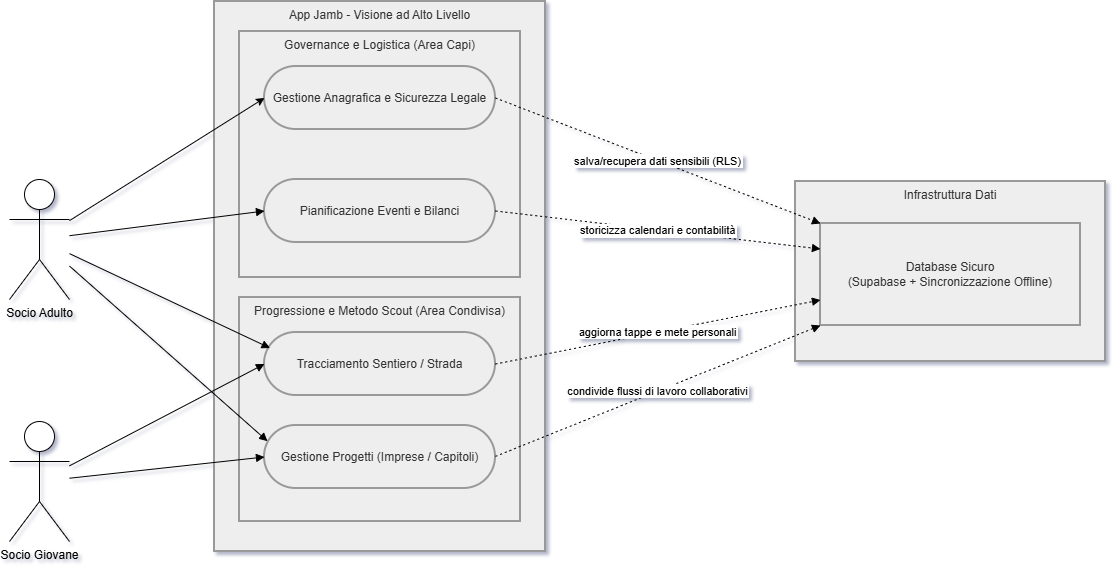
\includegraphics[width=15cm]{images/Use_Case_generale_Jamb.drawio.png}
  \caption{Diagramma dei casi d'uso ad alto livello del sistema Jamb.}
  \label{fig:usecase-generale}
\end{figure}

Il diagramma dei casi d'uso ad alto livello illustra la struttura fondamentale dell'ecosistema \textbf{\textit{Jamb}}, evidenziando la separazione tra le responsabilità amministrative e le dinamiche educative. L'architettura garantisce ai Soci Adulti l'accesso esclusivo ai moduli logistici, strumenti indispensabili per garantire la sicurezza legale, gestire la contabilità di unità o di gruppo e pianificare eventi.

Parallelamente, l'area dedicata al metodo scout si presenta come un ambiente collaborativo e interattivo: i Soci Giovani possono tracciare la propria progressione personale e gestire i loro progetti condivisi (come le Imprese o i Capitoli), mentre i capi intervengono con permessi mirati al monitoraggio del percorso. A fare da garante a questa divisione dei ruoli interviene l'infrastruttura dati esterna, la quale applica policy di sicurezza per isolare le informazioni sensibili e assicura, tramite la sincronizzazione asincrona, l'operatività del sistema anche durante le attività all'aperto prive di copertura di rete.

\newpage

\subsection{Descrizione principali attori}
L'ecosistema di \textbf{\textit{Jamb}} si divide in due macro-categorie, definite in base a come gli utenti vivono l'app nella loro quotidianità scout:


\textbf{Socio Adulto:} membro della Comunità Capi che accede al sistema per gestire l'operatività e la sicurezza della propria unità o dell'intero gruppo. Utilizza l'app per fare l'appello, consultare rapidamente schede mediche e documenti legali, rendicontare la cassa e validare il percorso educativo dei ragazzi.

\textbf{Socio Giovane:} utente protagonista del metodo scout (esploratore, guida, rover o scolta) che accede all'app per tracciare attivamente la propria crescita. A seconda della branca, la utilizza per monitorare il proprio Sentiero, gestire i materiali e le imprese di pattuglia, o redigere in totale privacy il proprio Punto della Strada.


\subsection{Elenco user stories}
Per tradurre le necessità operative in funzionalità concrete, il sistema è stato modellato attraverso le seguenti User Stories. L'elenco è organizzato seguendo rigorosamente la gerarchia dei permessi "a matrioska": si parte dalle interazioni base dell'Utente, passando per i ruoli operativi di branca (Capo e Aiuto/Capo Unità), fino ad arrivare alle viste aggregate delle figure di coordinamento (Capo Gruppo e Assistente Ecclesiastico).

Per guidare in modo efficiente le fasi di implementazione, a ciascuna User Story è stato inoltre assegnato un livello di priorità da 1 a 3, dove 1 indica un'estensione secondaria o futura, mentre 3 rappresenta una funzionalità critica e imprescindibile per il sistema.

\begin{figure}[h]
  \centering
  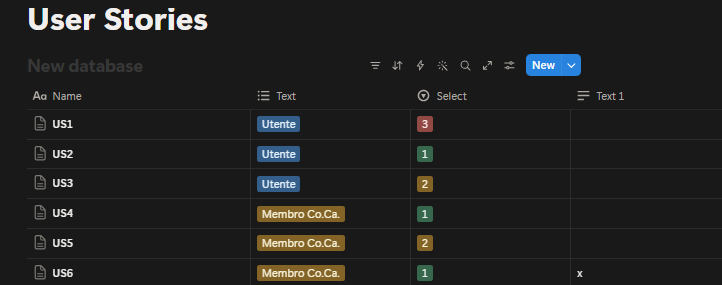
\includegraphics[width=15cm]{images/Screenshot 2026-04-14 100706.png}
  \caption{Panoramica dell'elenco delle user stories del progetto.}
  \label{fig:user-stories-overview}
\end{figure}

\newpage

\begin{enumerate}[label=\textbf{US\arabic*:}]
  \item Come Utente, voglio un'interfaccia facilmente intuibile e navigabile, così da riuscire a gestire tutto al meglio.
  \item Come Utente, voglio dei badge virtuali che rappresentino il mio storico all’interno dell’associazione, così che io possa avere uno storico della mia attività.
  \item Come Utente, voglio poter modificare le preferenze dell’app, così da rendere più personale l’esperienza sull’app.
  \item Come Capo, voglio i tasti delle funzioni più usate, così che velocizzo il mio lavoro.
  \item Come Capo, voglio un'agenda degli eventi riguardanti la Comunità Capi (Co.Ca.), così che non perdo nessun evento o riunione.
  \item Come Capo, voglio poter visualizzare a che punto mi trovo del mio iter formativo, così che mi possa rendere conto del mio progresso nella formazione.
  \item Come Capo, voglio avere a disposizione uno strumento per scrivere e tracciare il percorso del mio Progetto del Capo.
  \item Come Capo, voglio delle nozioni riguardanti il metodo della mia branca, così che io possa imparare facilmente ed essere sempre stimolato.
  \item Come Capo, voglio avere a disposizione in una sezione apposita tutti i documenti più importanti, come il patto associativo, lo statuto A.G.E.S.C.I., il metodo delle varie branche, così che io possa avere in un unico posto tutti i documenti spesso utili durante la progettazione delle varie attività.
  \item Come Capo, voglio un luogo dove tutta la Co.Ca. condivida i documenti che ogni Capo del gruppo deve vedere o avere sempre a disposizione.
  \item Come Aiuto Capo Unità, voglio poter visualizzare il progresso del Progetto Educativo di Gruppo (PEG), così che io possa tenere d’occhio quanto la mia branca si stia impegnando nel seguirlo e vedere i punti critici del PEG.
  \item Come Aiuto Capo Unità, voglio una lista di tutti i ragazzi appartenenti alla mia branca, con le informazioni più importanti come allergie e medicine vicino al nome del rispettivo ragazzo, così da tenere sotto controllo tutte le situazioni mediche dei ragazzi ed in caso di agire con prontezza.
  \item Come Aiuto Capo Unità, voglio una lista di numeri di emergenza da chiamare per ogni ragazzo, così da avere un contatto di riferimento a cui rivolgermi in caso di necessità.
  \item Come Aiuto Capo Unità, voglio avere sempre sottocontrollo quanta contabilità ha a disposizione la mia branca e voglio poter modificare il valore in base alle entrate ed uscite che affronto, così che ogni Capo della branca sappia la situazione economica costantemente aggiornata.
  \item Come Aiuto Capo Unità, voglio un calendario della branca visualizzabile solo dai Capi di quella specifica branca (non è un ulteriore calendario rispetto a quello della Co.Ca. ma si va a ”sommare”), così che ogni Capo della branca sappia tutti gli appuntamenti di quest’ultima.
  \item Come Aiuto Capo Unità, voglio un modo per tenere traccia delle presenze durante un qualsiasi evento, che possa essere una semplice riunione o un'uscita/campo, così da potermi accorgere dell’assenza ripetuta di qualche ragazzo ed agire tempestivamente.
  \item Come Aiuto Capo Unità, voglio avere a disposizione il Programma di Unità, così da poterlo consultare per la progettazione delle attività.
 \item Come Aiuto Capo Unità, voglio poter programmare un campo per la mia branca, avendo a disposizione la divisione per pattuglie e di poter vedere tutto ciò che le altre pattuglie hanno condiviso sull’applicazione, così da vedere a che punto lo Staff si trova con la progettazione del campo.
 \item Come Aiuto Capo Unità, voglio un luogo dove poter caricare e gestire tutti i documenti che la branca ha bisogno di condividere, così che io possa condividere e ricevere documenti utili con tutti i capi della branca.
 \item Come Aiuto Capo Unità, voglio avere una schermata per gestire i vari sotto gruppi di ogni branca (squadriglie, consiglio capi, consiglio della rupe, alta squadriglia), così da poter sfruttare al meglio questi strumenti del metodo.
 \item Come Aiuto Capo Unità, voglio poter gestire tutta la parte più burocratica che riguarda i ragazzi come i censimenti, privacy, schede mediche, di tutta la branca, così da poter monitorare la situazione in maniera costante e precisa.
 \item Come Aiuto Capo Unità, voglio un sistema di alert che mi avvisi della vicina scadenza di qualche documento burocratico, così da avere i documenti sottocontrollo.
 \item Come Aiuto Capo Unità, voglio vedere le informazioni del singolo ragazzo, così da poter vedere il suo storico ed adattarmi nel migliore dei modi.
 \item Come Capo Unità, voglio poter scrivere il programma di unità, così da poter seguire al meglio gli obiettivi del PEG.
 \item Come Capo Unità, voglio poter scrivere degli avvisi che tutti i capi della branca ricevano, così da gestire al meglio la comunicazione.
 \item Come Capo Unità, voglio uno strumento che mi aiuti a redigere il bilancio consolidato della branca, così che mi sia facilitato il compito complesso del dover redigere il bilancio.
 \item Come Capo Gruppo, voglio una lista di tutti i ragazzi del gruppo con la loro rispettiva situazione burocratica, così da poter sollecitare il Capo Unità rispettivo e tenere tutto sottocontrollo.
 \item Come Capo Gruppo, voglio un calendario con tutti gli eventi di ogni branca, così da conoscere gli appuntamenti di tutte le branche.
 \item Come Capo Gruppo, voglio poter tenere traccia dell’iter formativo di ogni Capo della Co.Ca., così da poter spronare i Capi nella loro formazione necessaria per offrire un servizio migliore ai ragazzi.
 \item Come Capo Gruppo, voglio poter scrivere e modificare il PEG, così da dare una direzione unica a tutto il gruppo.
 \item Come Capo Gruppo, voglio uno strumento che mi aiuti a redigere il bilancio consolidato del gruppo prendendo le informazione dai vari bilanci delle branche, così che mi sia facilitato il compito complesso del dover redigere il bilancio.
 \item Come Assistente Ecclesiastico, voglio uno strumento per la creazione delle veglie per le varie branche, così che mi sia più semplice la progettazione.
 \item Come Assistente Ecclesiastico, voglio poter scrivere delle pillole di spiritualità che la Co.Ca. e la branca R/S possano leggere.
 \item Come Assistente Ecclesiastico, voglio ricevere il punto della strada dei ragazzi R/S (solo se loro acconsentono).
\end{enumerate}

\newpage

\section{Fase Creativa ed Ideazione}
\subsection{Selezione dell'idea finale e motivazioni}
All'inizio della fase di progettazione sono state valutate diverse strade per cercare di coprire tutte le necessità del metodo scout, realizzando anche dei mockup per visualizzare come organizzare le varie schermate. In questa fase l'obiettivo era capire quali funzionalità fossero davvero utili per la vita quotidiana di un gruppo. Tuttavia, data la vastità del dominio e la mole di lavoro richiesta, è emerso che sviluppare da zero un'app completa per ogni singola branca e per ogni aspetto del metodo era troppo complesso per le tempistiche del progetto. È stato quindi necessario fare delle scelte per limitare le tempistiche, è stato quindi deciso di puntare su un MVP (Minimum Viable Product).  L'idea finale è stata quella di concentrarsi sulla parte gestionale e logistica dedicata ai Soci Adulti, includendo sia il livello di unità che quello di gruppo. Questa scelta nasce dalla consapevolezza che l'organizzazione e la burocrazia portano via molto tempo agli educatori. L'app deve quindi risolvere questo problema reale, permettendo di gestire in modo centralizzato le anagrafiche, i moduli medici e i documenti per la privacy di tutto il gruppo.  Per questo motivo, le funzionalità dedicate esclusivamente ai ragazzi (come la gestione del Sentiero, le Imprese o il Punto della Strada) sono state momentaneamente accantonate. Pur essendo idee molto valide per il futuro, è stato ritenuto fondamentale avere prima una base solida e funzionante per la parte amministrativa e di coordinamento tra le varie branche del gruppo.  In conclusione, l'app finale si concentra sul fornire ai Capi Unità e ai Capi Gruppo uno strumento affidabile per la gestione dei censimenti, dei bilanci e dei calendari condivisi. Questo approccio permette di testare con precisione la sincronizzazione offline e la sicurezza dei dati sensibili, garantendo una base robusta prima di espandere il sistema ad altre funzionalità.

\subsection{Mockup}
\subsubsection{Struttura generale dell'interfaccia}

\begin{center}
  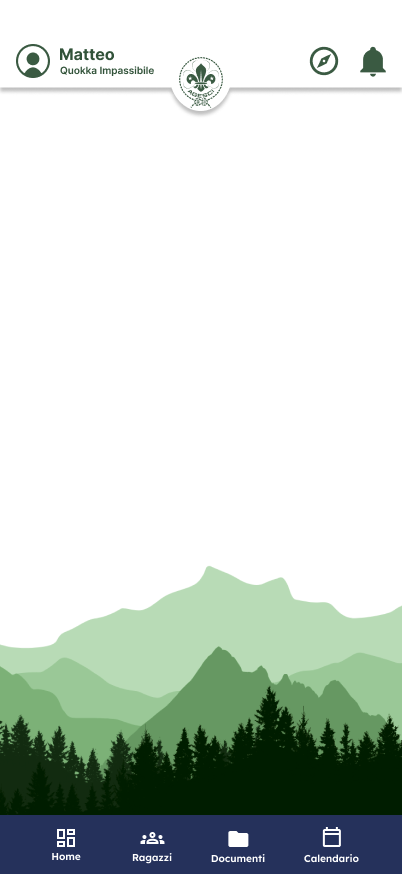
\includegraphics[width=0.32\textwidth]{images/iPhone 17 - sfondo vuoto.png}
  \captionof{figure}{Mockup della struttura generale dell'interfaccia con sfondo base dell'applicazione}
  \label{fig:mockup-struttura-generale}
\end{center}

Prima di spiegare nel dettaglio le varie schermate, è utile descrivere la struttura di base dell'applicazione, visibile nel mockup con lo sfondo vuoto (\textbf{Figura~\ref{fig:mockup-struttura-generale}}). L'interfaccia utente è stata progettata con un'impostazione fissa composta da due elementi principali: una barra in alto (Top Bar) e una barra di navigazione in basso (Bottom Navigation Bar). Questa scelta è stata fatta per far sì che l'utente abbia sempre dei punti di riferimento chiari e non si perda durante l'utilizzo dell'app.

La Bottom Navigation Bar serve appunto per la navigazione principale e permette all'utente di spostarsi rapidamente tra le quattro sezioni fondamentali dell'app. Troviamo il pulsante per la Home, quello per i Ragazzi (che porta alla lista dei censiti), la sezione Documenti e infine il Calendario. Avendo questa barra sempre presente sullo schermo, un Capo può passare dalla gestione di un'attività alla ricerca di un file in un attimo, senza dover tornare indietro in sottomenu complicati.

La Top Bar, invece, rimane fissa nella parte superiore. A sinistra presenta l'icona del profilo dell'utente, con il suo nome e il "totem" scout. Anche se per ora non ci sono dei mockup dedicati, l'idea di base è che cliccando lì l'utente venga rimandato alla sua pagina personale, centrata sulla propria formazione e sul Progetto del Capo. Al centro della barra c'è il logo dell'A.G.E.S.C.I., mentre sulla destra troviamo i pulsanti di servizio: l'icona della campanella serve per aprire la sezione delle notifiche, mentre l'icona a forma di bussola porta alle impostazioni dell'app. Usare una bussola al posto della solita rotellina degli ingranaggi è una scelta grafica pensata appositamente per richiamare il mondo e l'immaginario scout.

\subsubsection{Home screen e strumenti di gestione quotidiana}

\begin{figure}[ht]
  \centering
  \begin{subfigure}[t]{0.23\textwidth}
    \centering
    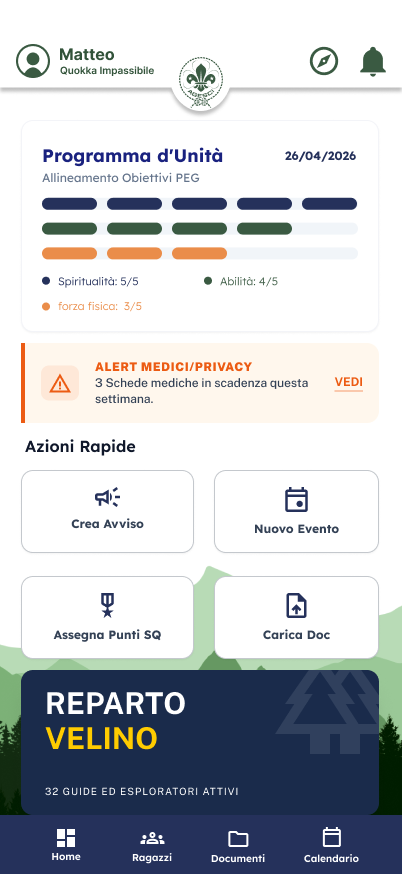
\includegraphics[width=\linewidth]{images/iPhone 17 - Home (1).png}
    \caption{Schermata Home dell'applicazione.}
    \label{fig:mockup-home}
  \end{subfigure}
  \hfill
  \begin{subfigure}[t]{0.23\textwidth}
    \centering
    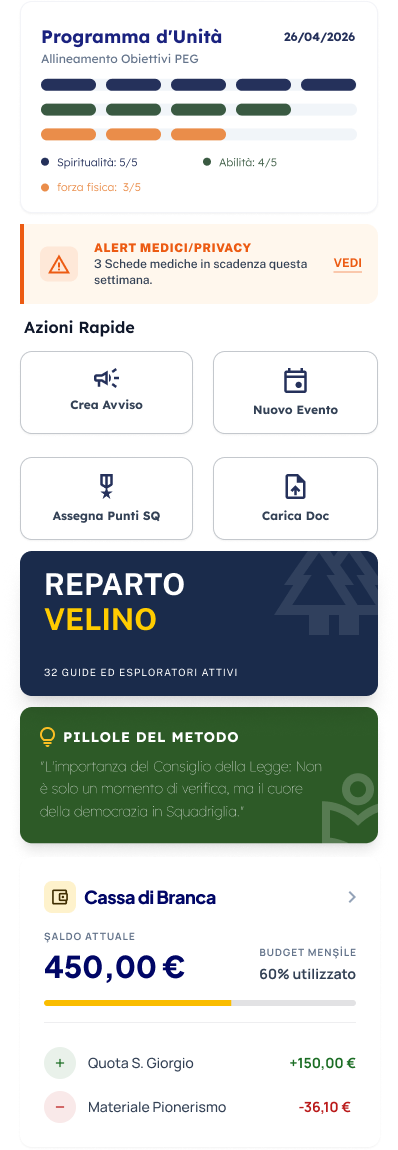
\includegraphics[width=\linewidth]{images/Frame 2.png}
    \caption{Tutti i widget presenti nella schermata Home.}
    \label{fig:mockup-frame2}
  \end{subfigure}
  \hfill
  \begin{subfigure}[t]{0.23\textwidth}
    \centering
    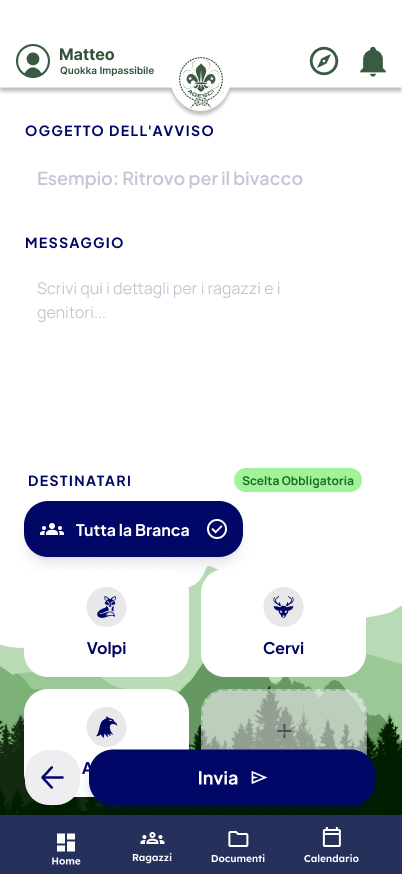
\includegraphics[width=\linewidth]{images/iPhone 17 - Creazione avviso.png}
    \caption{Interfaccia per la creazione di un avviso.}
    \label{fig:mockup-avviso}
  \end{subfigure}
  \hfill
  \begin{subfigure}[t]{0.23\textwidth}
    \centering
    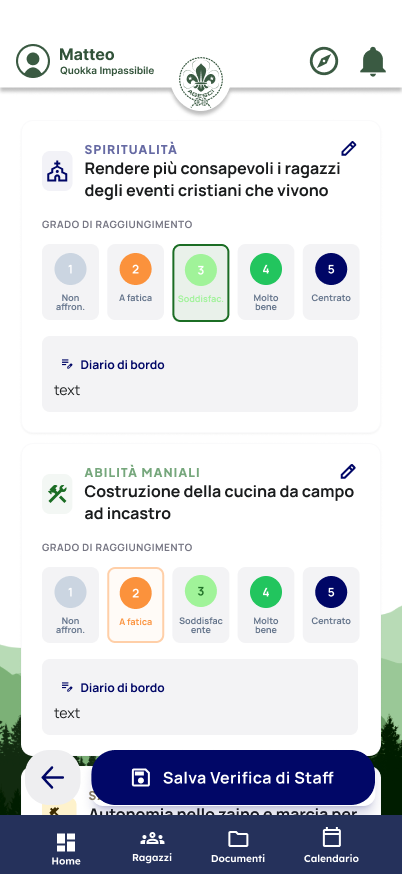
\includegraphics[width=\linewidth]{images/iPhone 17 - Modifica PEG.png}
    \caption{Vista di modifica del Programma d'Unità.}
    \label{fig:mockup-peg}
  \end{subfigure}
  \caption{Mockup principali dell'interfaccia di Jamb.}
  \label{fig:mockup-jamb}
\end{figure}

La schermata principale (\textbf{Figura~\ref{fig:mockup-jamb}\subref{fig:mockup-home}}) rappresenta la prima schermata appena si entra in \textbf{\textit{Jamb}}. Il design di questa interfaccia è stato concepito con un duplice obiettivo: fornire un colpo d'occhio immediato sulla salute della branca e ridurre al minimo i passaggi necessari per compiere le operazioni più frequenti. L'intera vista è strutturata a widget scorrevoli, organizzati per priorità d'uso.

Nella parte superiore della dashboard spicca il widget dedicato al Programma d'Unità, cioè al documento annuale con cui lo Staff declina per la propria branca gli obiettivi del Progetto Educativo di Gruppo. Il widget ne traduce visivamente l'avanzamento. Tramite indicatori grafici, il Capo può monitorare istantaneamente il bilanciamento delle aree educative, come formazione del carattere, salute e forza fisica, abilità manuale e servizio al prossimo. Da questo cruscotto si accede direttamente alla vista di modifica (\textbf{Figura~\ref{fig:mockup-jamb}\subref{fig:mockup-peg}}), dove lo Staff può valutare periodicamente il grado di raggiungimento degli obiettivi e compilare il diario di bordo.

Un elemento di fondamentale importanza per la gestione del rischio è il banner degli alert. Posizionato in alto per catturare subito l'attenzione, questo indicatore segnala le urgenze, come ad esempio le schede mediche o i moduli privacy in scadenza, permettendo allo Staff di intervenire tempestivamente prima di un'uscita. Subito sotto, l'interfaccia presenta una griglia di azioni rapide, vere e proprie scorciatoie pensate per l'operatività sul campo, come la creazione di un nuovo evento, il caricamento di un documento o l'assegnazione dei punti per la classifica tra le squadriglie. Tra queste, la funzione di creazione degli avvisi apre un modulo ottimizzato (\textbf{Figura~\ref{fig:mockup-jamb}\subref{fig:mockup-avviso}}) per la comunicazione interna che permette di segmentare i destinatari, inviando il messaggio all'intero Reparto o a singole Squadriglie.

Scorrendo l'interfaccia, dopo il riepilogo visivo dei censiti attivi, si incontrano due ulteriori sezioni pensate per il supporto metodologico e logistico. Da una parte, il widget dedicato alle pillole del metodo offre uno spazio ideato per fornire continui spunti di riflessione, ad esempio sull'importanza del Consiglio della Legge, supportando così la formazione personale dell'educatore in modo leggero e costante ad ogni apertura dell'applicazione. Dall'altra, la sezione dedicata alla cassa di branca fornisce un estratto rapido della situazione finanziaria dell'unità. Quest'ultimo blocco mostra a colpo d'occhio il saldo attuale, le ultimissime transazioni effettuate, come le entrate per le quote o le uscite per i materiali. In questo modo, l'educatore ha un'immediata consapevolezza delle risorse a disposizione senza dover necessariamente navigare nella sezione amministrativa completa.

\subsubsection{Gestione anagrafica e sicurezza}

\begin{figure}[H]
  \centering
  \begin{subfigure}[t]{0.31\textwidth}
    \centering
    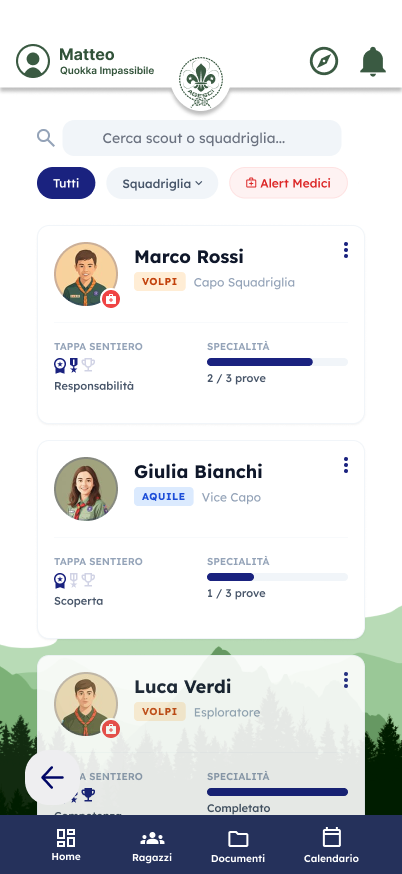
\includegraphics[width=\linewidth]{images/iPhone 17 - Ragazzi.png}
    \caption{Elenco dei ragazzi dell'unità con filtri e indicatori rapidi.}
    \label{fig:mockup-ragazzi}
  \end{subfigure}
  \hfill
  \begin{subfigure}[t]{0.31\textwidth}
    \centering
    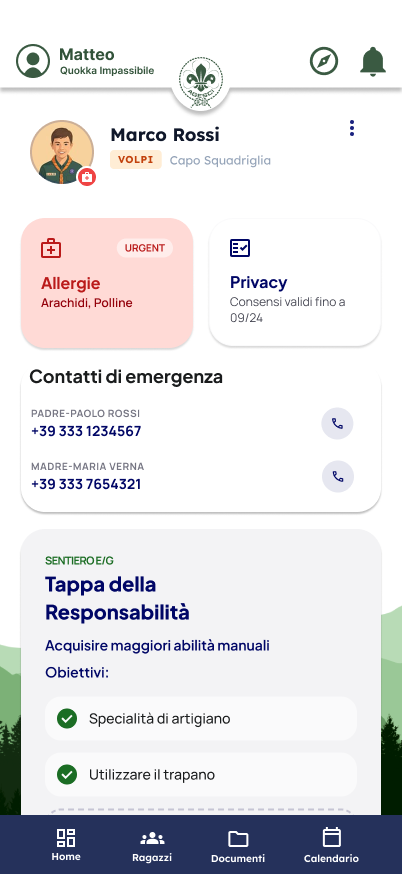
\includegraphics[width=\linewidth]{images/iPhone 17 - Singolo ragazzo.png}
    \caption{Scheda di dettaglio del singolo ragazzo.}
    \label{fig:mockup-singolo-ragazzo}
  \end{subfigure}
  \hfill
  \begin{subfigure}[t]{0.31\textwidth}
    \centering
    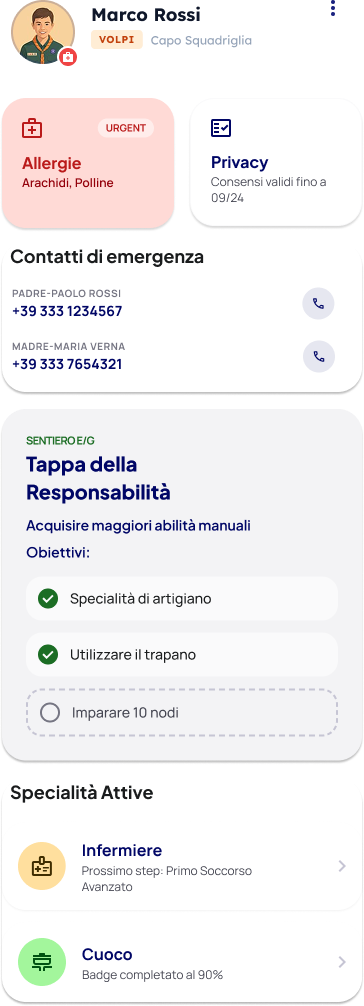
\includegraphics[width=\linewidth]{images/Frame 6.png}
    \caption{Tutti i widget della schermata di dettaglio del singolo ragazzo.}
    \label{fig:mockup-frame6}
  \end{subfigure}
  \caption{Mockup della sezione anagrafica e sicurezza di Jamb.}
  \label{fig:mockup-anagrafica-sicurezza}
\end{figure}

La seconda macro-area dell'applicazione è dedicata alla consultazione dell'anagrafica, con un design fortemente orientato alla minimizzazione dei rischi e al monitoraggio educativo individuale. La schermata principale di questa sezione (\textbf{Figura~\ref{fig:mockup-anagrafica-sicurezza}\subref{fig:mockup-ragazzi}}) presenta l'elenco completo dei ragazzi appartenenti all'unità. Per ottimizzare i tempi di ricerca, specialmente durante le attività all'aperto, l'interfaccia integra una barra di ricerca testuale e una serie di filtri rapidi, i quali permettono di segmentare la lista per singola squadriglia o di isolare unicamente i profili che presentano criticità sanitarie. Ogni censito è rappresentato da una scheda riassuntiva (\textbf{Figura~\ref{fig:mockup-anagrafica-sicurezza}\subref{fig:mockup-singolo-ragazzo}}) che indica la squadriglia e il ruolo ricoperto, offrendo contemporaneamente un primo colpo d'occhio sull'avanzamento del Sentiero e sulle prove di specialità. A livello visivo, un elemento di primaria importanza per la prevenzione è l'icona a forma di valigetta rossa: questo indicatore segnala immediatamente la presenza di esigenze mediche, garantendo un'allerta preventiva ancor prima di aprire il profilo del ragazzo.

Accedendo al dettaglio del singolo censito, l'educatore entra in una vera e propria cartella personale digitale, la cui architettura dell'informazione è studiata per dare priorità assoluta alla sicurezza. La porzione superiore della schermata ospita infatti i widget dedicati alla tutela sanitaria e legale. Un modulo evidenziato in rosso riporta esplicitamente le urgenze mediche, specificando nel dettaglio le eventuali allergie alimentari o ambientali per prevenire incidenti durante i pasti al campo. Accanto ad esso, un indicatore monitora la scadenza della validità dei consensi per la privacy. Immediatamente sotto, il sistema posiziona in grande evidenza i contatti di emergenza dei genitori, integrando dei pulsanti di chiamata rapida che permettono allo Staff di mettersi in contatto con le famiglie in pochissimi istanti e senza dover abbandonare l'applicazione.

La metà inferiore del profilo sposta invece il focus sull'aspetto metodologico, fungendo da strumento di tracciamento per la progressione personale. Un blocco interattivo dedicato al Sentiero illustra la Tappa attualmente vissuta dal ragazzo, declinandola in obiettivi pratici e verificabili tramite un sistema di spunte. Questa struttura permette al Capo di validare sul momento il superamento di una prova, come l'acquisizione di un'abilità manuale. Infine, l'interfaccia si conclude con la sezione relativa alle specialità attive, dove è possibile monitorare lo stato di avanzamento e i prossimi passi necessari per il conseguimento dei vari badge di competenza, trasformando la scheda del ragazzo in un vero e proprio diario di bordo per la sua crescita educativa.

\newpage

\subsubsection{Archiviazione documenti e gestione burocratica}

\begin{figure}[H]
  \centering
  \begin{subfigure}[t]{0.23\textwidth}
    \centering
    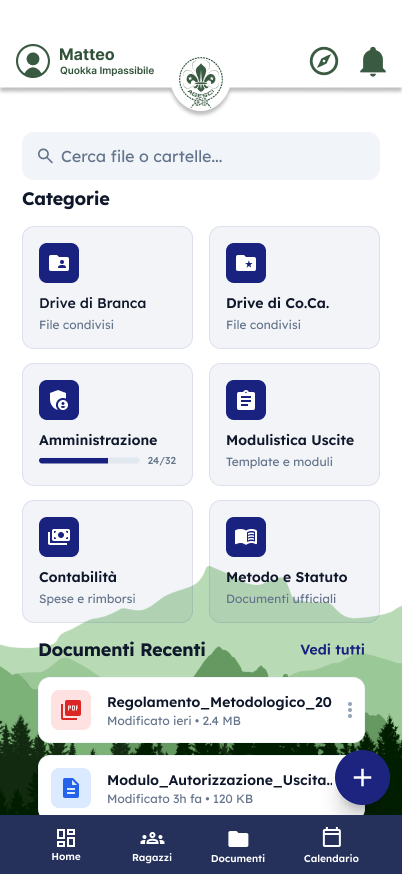
\includegraphics[width=\linewidth]{images/iPhone 17 - Documenti.png}
    \caption{Hub principale della sezione documentale.}
    \label{fig:mockup-documenti}
  \end{subfigure}
  \hfill
  \begin{subfigure}[t]{0.23\textwidth}
    \centering
    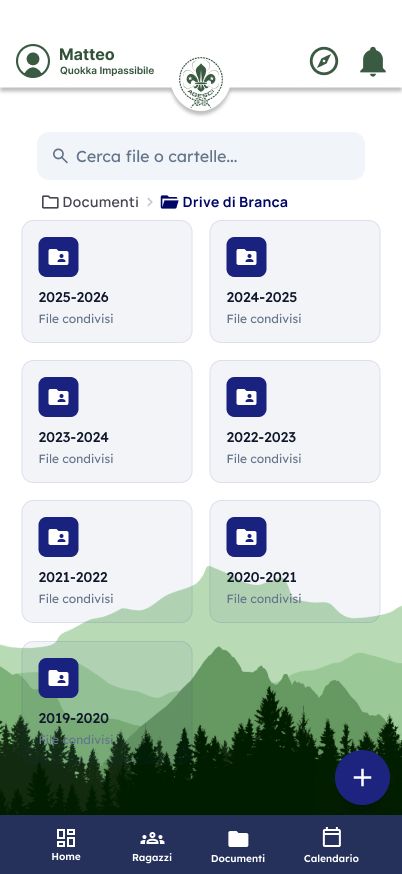
\includegraphics[width=\linewidth]{images/iPhone 17 - Drive di branca.png}
    \caption{Accesso al Drive di Branca.}
    \label{fig:mockup-drive-di-branca}
  \end{subfigure}
  \hfill
  \begin{subfigure}[t]{0.23\textwidth}
    \centering
    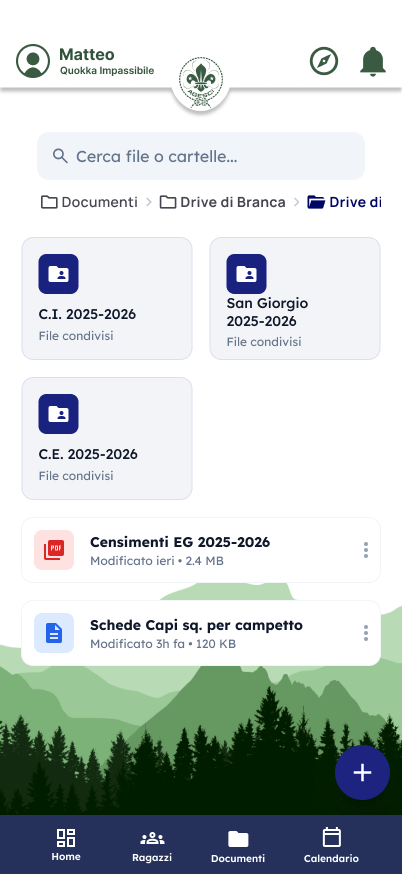
\includegraphics[width=\linewidth]{images/iPhone 17 - Drive 2025-2026.png}
    \caption{Esplorazione delle cartelle dell'anno scout 2025--2026.}
    \label{fig:mockup-explorer}
  \end{subfigure}
  \hfill
  \begin{subfigure}[t]{0.23\textwidth}
    \centering
    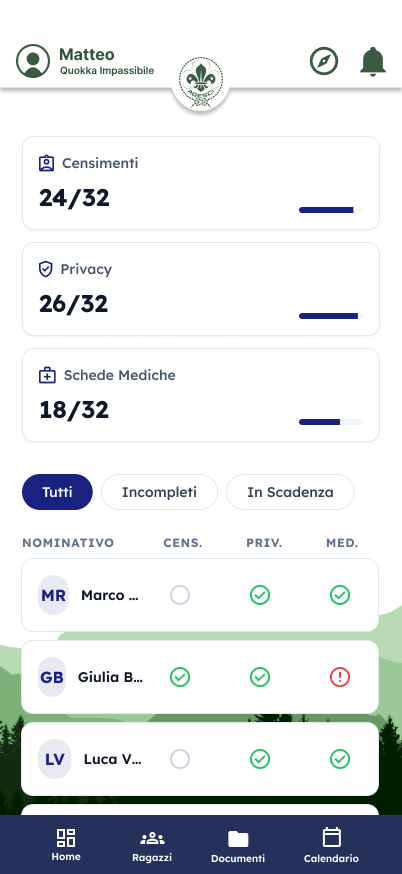
\includegraphics[width=\linewidth]{images/iPhone 17 - Checklist documenti.png}
    \caption{Checklist amministrativa con stato dei documenti.}
    \label{fig:mockup-burocrazia}
  \end{subfigure}
  \caption{Mockup della sezione di archiviazione documentale e gestione burocratica di Jamb.}
  \label{fig:mockup-documenti-burocrazia}
\end{figure}

La terza macro-area dell'applicazione funge da vero e proprio archivio centrale, accessibile dalla barra di navigazione inferiore. L'hub principale (\textbf{Figura~\ref{fig:mockup-documenti-burocrazia}\subref{fig:mockup-documenti}}) suddivide l'area di lavoro in categorie logiche distinte, mettendo in evidenza nella parte inferiore gli ultimi file aperti per ridurre i tempi di ricerca. L'infrastruttura di archiviazione si suddivide nei Drive condivisi, separati in "Drive di Branca" (\textbf{Figura~\ref{fig:mockup-documenti-burocrazia}\subref{fig:mockup-drive-di-branca}-\subref{fig:mockup-explorer}}) e "Drive di Co.Ca.". Queste aree si presentano visivamente come un file explorer tradizionale, permettendo agli utenti di navigare in modo intuitivo tra cartelle organizzate per anni scout o per specifici eventi. L'ecosistema si completa con l'area "Modulistica Uscite", pensata per i template standardizzati per presenze e programmi, e la sezione "Metodo e Statuto", che funge da biblioteca per i documenti associativi ufficiali.

Strettamente legata alla documentazione è la sezione relativa all'Amministrazione (\textbf{Figura~\ref{fig:mockup-documenti-burocrazia}\subref{fig:mockup-burocrazia}}), che fornisce all'educatore un cruscotto interattivo per tenere sotto controllo i documenti legali dell'unità. L'interfaccia presenta nella parte superiore tre barre di avanzamento che mostrano a colpo d'occhio lo stato di raccolta dei censimenti, dei moduli privacy e delle schede mediche. Al di sotto, una lista nominativa permette di monitorare la situazione di ogni singolo ragazzo attraverso un sistema di indicatori circolari che si aggiornano automaticamente in base alle date registrate. Questo meccanismo visivo a semaforo utilizza il colore verde per indicare una documentazione perfettamente in regola, il giallo per avvisare preventivamente di un documento in scadenza e il rosso per segnalare un elemento del tutto mancante o già scaduto. Sfruttando questa classificazione automatica, i filtri consentono di isolare i profili che richiedono attenzione, supportando lo Staff nel prevenire tempestivamente qualsiasi scopertura legale o assicurativa senza dover effettuare verifiche manuali.

\subsubsection{Gestione finanziaria}

\begin{figure}[H]
  \centering
  \begin{subfigure}[t]{0.31\textwidth}
    \centering
    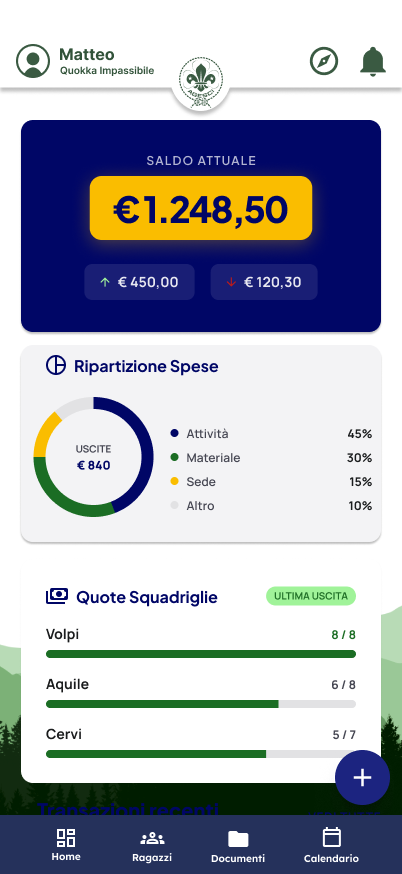
\includegraphics[width=\linewidth]{images/iPhone 17 - Sezione contabile.png}
    \caption{Dashboard della sezione contabile con saldo e riepilogo delle spese.}
    \label{fig:mockup-sezione-contabile}
  \end{subfigure}
  \hfill
  \begin{subfigure}[t]{0.31\textwidth}
    \centering
    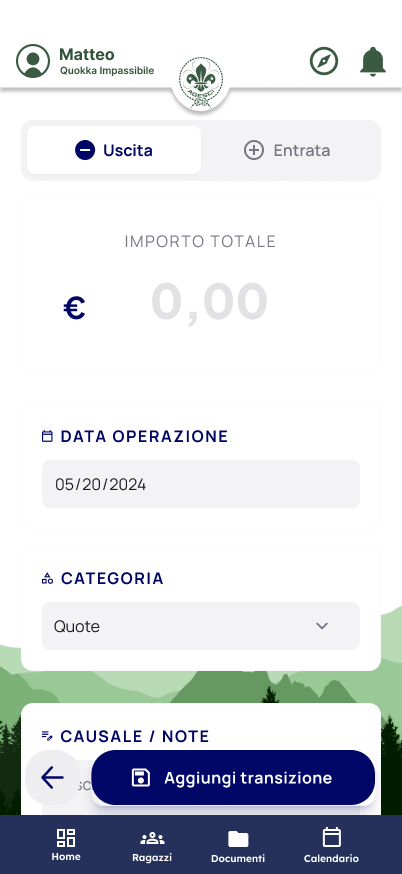
\includegraphics[width=\linewidth]{images/iPhone 17 - Form transazione.png}
    \caption{Form per l'inserimento di una nuova transazione economica.}
    \label{fig:mockup-form-transazione}
  \end{subfigure}
  \hfill
  \begin{subfigure}[t]{0.31\textwidth}
    \centering
    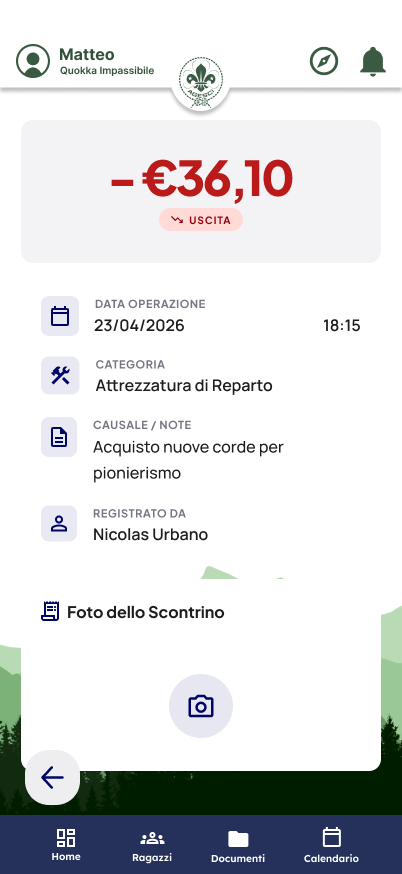
\includegraphics[width=\linewidth]{images/iPhone 17 - Specifiche transazione.png}
    \caption{Vista di dettaglio di una singola transazione registrata.}
    \label{fig:mockup-specifiche-transazione}
  \end{subfigure}
  \caption{Mockup della sezione di gestione finanziaria di Jamb.}
  \label{fig:mockup-gestione-finanziaria}
\end{figure}

Un'area di rilievo, comunque legata alla gestione dei documenti e della burocrazia, è dedicata interamente alla contabilità, un modulo progettato per sostituire l'uso frammentario di fogli di calcolo cartacei e digitali, garantendo massima trasparenza all'interno della pattuglia direttiva. La dashboard finanziaria accoglie l'utente evidenziando in modo chiaro il saldo attuale (\textbf{Figura~\ref{fig:mockup-gestione-finanziaria}\subref{fig:mockup-sezione-contabile}}), per poi scendere nel dettaglio analitico attraverso un grafico a ciambella che illustra la ripartizione percentuale delle uscite suddivise per categorie, come le spese per le attività o per l'acquisto di materiale. A completare questa panoramica è presente un indicatore visivo dedicato allo stato di raccolta delle quote da parte delle singole squadriglie.

L'interazione attiva avviene tramite il pulsante di aggiunta, che apre un modulo (\textbf{Figura~\ref{fig:mockup-gestione-finanziaria}\subref{fig:mockup-form-transazione}}) per la registrazione istantanea di nuove entrate o uscite. Il form richiede l'inserimento dell'importo, della data, della categoria e della causale, offrendo inoltre l'opportunità di digitalizzare il processo allegando direttamente la fotografia dello scontrino fiscale. Infine, selezionando una specifica transazione dallo storico, si accede a una schermata di dettaglio (\textbf{Figura~\ref{fig:mockup-gestione-finanziaria}\subref{fig:mockup-specifiche-transazione}}) che riepiloga tutte le informazioni inserite, indicando esplicitamente quale membro dello Staff ha registrato l'operazione, assicurando così una totale tracciabilità economica e facilitando la stesura del bilancio consolidato di fine anno.

\subsubsection{Pianificazione e calendario di gruppo}

\begin{figure}[H]
  \centering
  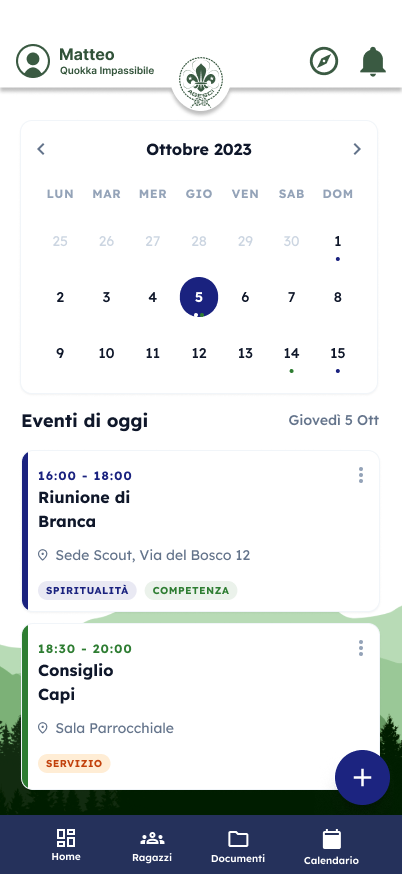
\includegraphics[width=0.34\textwidth]{images/iPhone 17 - Calendario.png}
  \caption{Mockup del calendario condiviso di gruppo con vista mensile ed eventi del giorno.}
  \label{fig:mockup-calendario}
\end{figure}

L'ultima macro-area dell'applicazione riguarda il Calendario, che funge da strumento principale per la pianificazione di tutte le attività. Si tratta di un calendario condiviso a livello di intero Gruppo, una scelta pensata per evitare sovrapposizioni tra le varie branche e permettere a ogni Capo di sapere cosa stanno facendo le altre unità. La schermata (\textbf{Figura~\ref{fig:mockup-calendario}}) è divisa in due parti: in alto c'è la classica griglia mensile per selezionare il giorno, mentre in basso compare la lista degli "Eventi di oggi" con tutti i dettagli necessari.

Una delle funzioni più utili di questa sezione è legata alla creazione di un nuovo evento. Quando lo Staff decide di inserire un'uscita o un campo, il sistema mette a disposizione automaticamente i template standardizzati che abbiamo già visto nella sezione "Modulistica Uscite" dei documenti. In questo modo, l'app aiuta i capi a non dimenticare nulla, fornendo già i modelli pronti per il menu, la tabella delle presenze e il programma dell'attività, collegando così la parte di pianificazione con quella dell'archivio documentale.

Dalla schermata si nota come ogni evento sia descritto in modo completo, riportando l'orario, il luogo dell'appuntamento (come la Sede Scout) e il titolo dell'incontro. Un dettaglio molto importante è la presenza di etichette colorate poste sotto ogni evento (altro non sono che gli obiettivi del Programma d'Unità). Queste etichette non sono solo dei semplici tag, ma servono a ricordare allo Staff quali obiettivi si stanno toccando con quella specifica attività, mantenendo la programmazione sempre coerente con gli obiettivi educativi fissati all'inizio dell'anno. Infine, tramite il pulsante flottante con il simbolo "+" in basso a destra, è possibile aggiungere nuovi appuntamenti in modo rapido, rendendo la gestione del tempo semplice e immediata per tutto il gruppo.

\section{Organizzazione del Lavoro}

Questo capitolo descrive come è stato condotto lo sviluppo, con quali strumenti e in quali tempi.

\subsection{Struttura del team e conseguenze sul processo}

Il progetto è stato svolto individualmente. La circostanza non è neutra rispetto al metodo, perché rende impossibili alcune pratiche per cui sono previste più persone, in particolare la revisione incrociata del codice e la suddivisione dei compiti. Sono stati adottati due approcci, la separazione del lavoro su rami dedicati, che obbliga a rileggere l'insieme delle modifiche prima di integrarle, e i test automatici sulla logica, che offrono un controllo indipendente dal giudizio di chi ha scritto il codice.

\subsection{I due cicli di sviluppo}

Il lavoro si è articolato in due cicli distinti, separati da una sospensione dettata dalla sessione d'esami. Ciascuno è durato poco più di una settimana e si è chiuso con un incremento funzionante.

Il primo ciclo, dal 28 aprile al 6 maggio, aveva come obiettivo la costruzione dell'interfaccia completa e la separazione della logica dalla presentazione, e si è chiuso con tutte le schermate navigabili su dati locali e con l'architettura a livelli già in piedi. Ho proceduto per aree funzionali, nell'ordine in cui compaiono nella navigazione, barra superiore e inferiore, avanzamento del Programma d'Unità, schermata principale, anagrafica dei ragazzi con il dettaglio individuale, specialità e brevetti, documenti e infine contabilità. Costruite le schermate, le ultime giornate sono state dedicate a due interventi di riorganizzazione, l'estrazione del livello di dominio e il passaggio dei widget a un modello con ViewModel e repository reattivi.

Il secondo ciclo, dall'11 al 18 luglio, aveva per obiettivo la sostituzione della sorgente dati con un backend reale e il collaudo della logica, e ha prodotto autenticazione, gestione della sessione, cinque repository migrati su Supabase e la suite di test automatici. Non ha aggiunto schermate, ha sostituito ciò che stava sotto, le implementazioni su file locali sono state affiancate da implementazioni su Supabase e attivate al posto delle precedenti cambiando una riga nel contenitore delle dipendenze. Nella stessa fase sono state corrette le anomalie emerse dal test con gli utenti, descritto nel capitolo dedicato al collaudo.

\subsection{Gestione del codice sorgente}

Il versionamento è affidato a Git, con repository remoto su GitHub. Il ramo principale è stato mantenuto sempre in uno stato compilabile, e ogni lavorazione è avvenuta su un ramo separato, riportato sul principale solo a lavorazione conclusa.

I rami seguono una convenzione basata sulla natura dell'intervento. Il prefisso \texttt{feature} indica l'aggiunta di una funzionalità e ne riporta l'area, come \texttt{feature/home}, \texttt{feature/ragazzi} e \texttt{feature/documenti}. Lo stesso prefisso è stato usato per i livelli architetturali introdotti come unità autonome, \texttt{feature/domain-layer} e \texttt{feature/data-layer}. Il prefisso \texttt{refactor} distingue gli interventi che riorganizzano codice esistente senza aggiungere funzionalità, come \texttt{refactor/ui-layer}. Il ramo \texttt{pre-release} è stato usato per consolidare la versione distribuita agli utenti per il collaudo.

\subsection{Strumenti}

Lo sviluppo è avvenuto su Antigravity con l'estensione Flutter, e le prove sono state condotte su emulatore Android e su dispositivo fisico. Il versionamento usa Git e GitHub. Lo schema del database, le policy di sicurezza e i dati di prova sono stati gestiti direttamente dalla console di Supabase, con l'editor SQL integrato. La distribuzione agli utenti per il collaudo è avvenuta tramite file \texttt{.apk} inviato tramite WhatsApp, come descritto nel capitolo sul collaudo.

Non sono stati adottati strumenti di project management collaborativo. Per un lavoro individuale una bacheca di attività avrebbe aggiunto un adempimento senza aggiungere coordinamento, e il tracciamento dell'avanzamento è stato affidato alla cronologia dei commit.

\subsection{Impegno orario}

Il primo ciclo di sviluppo è valutabile attorno alle cinquantacinque ore, il secondo attorno alle quarantacinque, per un totale di cento ore dedicate al codice. A queste si aggiungono circa dieci ore di analisi e progettazione della base di dati e delle policy di sicurezza, e altre quindici per la redazione della documentazione, portando l'impegno complessivo intorno alle centoventicinque ore.

Le due voci finali non compaiono nella cronologia del repository, perché riguardano lavoro svolto al di fuori dell'IDE, la progettazione della base di dati e delle policy si trova nella console di Supabase, mentre analisi e documentazione sono esterne al codice.

\section{Architettura di Sistema e Tecnologie}

Questo capitolo descrive la struttura software di \textbf{\textit{Jamb}}, illustrando le motivazioni delle scelte riguardanti le tecnologie impiegate, del pattern architetturale e delle librerie esterne.

\subsection{Stack Tecnologico e Pacchetti Esterni}

L'implementazione dell'app si basa su due pilastri tecnologici fondamentali; \textbf{Flutter} per il frontend e \textbf{Supabase} come backend. Questa combinazione è stata scelta per ottimizzare la produttività di un singolo sviluppatore, cercando di mantenere prestazioni elevate e costi contenuti.

\textbf{Flutter} è il framework di sviluppo, basato sul linguaggio \textbf{Dart}, utilizzato per la costruzione dell'interfaccia. La sua caratteristica fondamentale è la \textit{cross-platform} che permette, con una sola base di codice, di generare applicazioni native per Android e iOS, ottimizzando i tempi di sviluppo.

\textbf{Supabase} costituisce invece il backend. Costruito attorno ad un database relazionale \textbf{PostgreSQL}, che fornisce il servizio di autenticazione (Supabase Auth), le API di accesso ai dati e, soprattutto, il motore di \textit{Row Level Security} che avrà un capitolo dedicato.

A completare lo stack tecnico troviamo un insieme di pacchetti esterni, selezionati in base alle necessità delle parti integrate:
\begin{itemize}[topsep=0.5pt]
  \item \textbf{supabase\_flutter}: client ufficiale di Supabase, gestisce l'autenticazione, le query al database.
  \item \textbf{provider}: libreria di \textit{state management}, si occupa dell'iniezione delle dipendenze e della propagazione reattiva dei cambiamenti di stato all'interfaccia.
  \item \textbf{intl} e \textbf{flutter\_localizations}: gestiscono la localizzazione in lingua italiana e la formattazione di date e valute secondo le convenzioni locali.
  \item \textbf{table\_calendar}: fornisce il widget di calendario mensile interattivo utilizzato nella sezione di pianificazione degli eventi.
  \item \textbf{file\_picker} e \textbf{image\_picker}: consentono la selezione di documenti dal dispositivo e l'acquisizione di immagini, impiegate rispettivamente nel drive documentale e nell'allegato delle ricevute contabili.
  \item \textbf{flutter\_svg}: permette il rendering di grafica vettoriale, usata per i loghi istituzionali e le icone dell'applicazione.
  \item \textbf{url\_launcher}: abilita l'apertura di risorse esterne, come l'avvio diretto di una chiamata verso i contatti di emergenza dei ragazzi.
\end{itemize}

La combinazione di questi strumenti definisce un ecosistema moderno e manutenibile, in cui ogni dipendenza ha il proprio scopo, evitando l'introduzione di librerie futili.

\subsection{Pattern Architetturali}

La gestione di un dominio come quello scout, unita alla necessità di poter modificare la sorgente dei dati senza riscrivere l'interfaccia, ha reso indispensabile adottare fin dall'inizio un'architettura strutturata. La scelta è stata un'\textbf{architettura a livelli} (\textit{Layered Architecture}) organizzata secondo il pattern \textbf{MVVM} (Model-View-ViewModel).

Il codice è suddiviso in tre livelli, ciascuno con responsabilità nettamente separate e comunicanti solo con quello immediatamente adiacente:
\begin{itemize}[topsep=0.5pt]
  \item \textbf{Livello UI:} contiene le \textit{View} (i widget) e i \textit{ViewModel}. È organizzato \textit{per funzionalità}, poiché ogni schermata possiede esattamente una View e un ViewModel corrispondente.

  \item \textbf{Livello Domain:} ospita le entità di dominio (\texttt{Scout}, \texttt{Transazione}, \texttt{Evento}, \texttt{Obiettivo}, \texttt{Documento}) e, soprattutto, le \textbf{interfacce} dei repository. È il livello più stabile e non dipende da nessun altro.

  \item \textbf{Livello Data:} contiene le implementazioni concrete dei repository, ovvero l'unico punto del sistema che conosce Supabase. È organizzato \textit{per tipo}, dato che un repository viene utilizzato trasversalmente da più funzionalità.

\end{itemize}

All'interno del livello UI, il pattern MVVM stabilisce una divisione precisa dei compiti. La \textbf{View} si limita a mostrare lo stato che riceve e a inoltrare le interazioni dell'utente, senza contenere alcuna logica di business. Il \textbf{ViewModel} è invece una classe Dart che contiene la logica di presentazione, mantiene lo stato della schermata e dialoga con il livello dati. Questa separazione fa sì che, ad esempio, il calcolo del totale della cassa o il filtraggio dell'elenco dei ragazzi si trovino in classi indipendenti dai widget, e siano quindi verificabili singolarmente.

Il collegamento tra il livello UI e quello dati avviene tramite il \textbf{Repository Pattern} applicato secondo il principio di \textit{inversione delle dipendenze}. I ViewModel non conoscono mai le classi concrete che interrogano il database: dipendono esclusivamente dalle interfacce dichiarate nel livello di dominio (ad esempio \texttt{IScoutRepository}), mentre l'implementazione effettiva viene scelta e iniettata al momento dell'avvio dell'applicazione. Questo dettaglio è ciò che ha reso possibile la migrazione dell'intera applicazione: il passaggio da una gestione dei dati su file JSON, utile per i primi test, al backend Supabase ha richiesto unicamente la sostituzione dell'implementazione registrata, senza modificare né i ViewModel né alcun widget.

L'infrastruttura che rende operativo questo schema è la libreria \textbf{Provider}, che assolve contemporaneamente a due funzioni. In primo luogo agisce da contenitore per l'iniezione delle dipendenze: all'avvio dell'applicazione tutti i repository, i ViewModel e il servizio di sessione vengono registrati in cima all'albero dei widget e resi disponibili a qualsiasi componente sottostante, evitando di doverli propagare manualmente. In secondo luogo gestisce la propagazione dello stato, i ViewModel estendono ChangeNotifier e, ogni volta che il loro stato cambia, notificano gli osservatori, i quali ricostruiscono automaticamente le sole porzioni di interfaccia interessate.

Avremo quindi un \textbf{flusso di dati unidirezionale}: l'utente interagisce con la View, che inoltra l'evento al ViewModel; questo elabora la richiesta appoggiandosi al repository, aggiorna il proprio stato e notifica il cambiamento, provocando la ricostruzione dell'interfaccia. Il meccanismo è stato inoltre esteso ai repository stessi, resi anch'essi osservabili: quando un dato viene modificato sul database, il repository notifica i ViewModel in ascolto, che ricaricano le informazioni aggiornate.

\begin{figure}[H]
  \centering
  \includegraphics[width=0.4\textwidth]{images/pipeline.drawio (1).png}
  \caption{Pipeline dei dati tra i livelli dell'architettura}
  \label{fig:pipeline-layer}
\end{figure}

L'adozione di questo impianto architetturale è costata inizialmente in termini di file e di astrazioni, ma è stata ampiamente ripagata da due vantaggi: la \textbf{sostituibilità} di un singolo layer, come nel caso della sorgente dati, con la migrazione verso Supabase, e la \textbf{testabilità} della logica applicativa, che ha permesso di verificare i ViewModel utilizzando repository simulati in memoria, come verrà illustrato nel capitolo dedicato al testing.

\subsection{Paradigma Offline-First}

Tra tutti i requisiti tecnici emersi dall'analisi del dominio, la possibilità di usare \textbf{\textit{Jamb}} in assenza di rete è quello più fondamentale per la realtà d'uso. Le attività scout si svolgono in ambienti privi di rete: campi estivi in aree boschive, route di più giorni in montagna, uscite in luoghi isolati. Sono esattamente le situazioni in cui l'accesso ai dati critici, come le schede mediche o i contatti di emergenza, risulta essenziale. Un'applicazione che smette di funzionare proprio in quelle circostanze fallirebbe nel suo obiettivo primario, motivo per cui il paradigma \textit{offline-first} è stato posto fin dall'inizio tra i pilastri architetturali del progetto.

L'architettura progettata per soddisfare questo requisito si articola su tre componenti. Il database remoto \textbf{PostgreSQL} gestito su Supabase costituisce la fonte di verità condivisa tra tutti i dispositivi. Su ciascun dispositivo è previsto un database locale \textbf{SQLite}, che l'applicazione interroga direttamente: in questo modo ogni lettura e ogni scrittura avvengono istantaneamente in locale, indipendentemente dalla presenza o no della rete. A fare da collegamento tra i due interviene \textbf{PowerSync}, un motore di sincronizzazione progettato specificamente per integrarsi con Supabase, che si occupa di replicare le modifiche in entrambe le direzioni non appena la rete viene ripristinata e di applicare le regole di risoluzione dei conflitti nel caso in cui lo stesso dato sia stato modificato da più utenti mentre erano disconnessi.

La differenza sostanziale rispetto a un approccio basato su una semplice cache è che, in un modello offline-first, l'assenza di rete non rappresenta una condizione di errore da gestire ma lo stato ordinario di funzionamento: l'interfaccia non deve aspettare nessuna risposta remota, dato che legge sempre dal database locale, mentre la sincronizzazione avviene in background e in modo trasparente per l'utente.


Purtroppo è necessario precisare che, nella versione MVP, questa feature non è stata implementata: l'applicazione interagisce direttamente con Supabase e richiede pertanto una connessione. La scelta di rinviare questo componente è stata volontaria ed è causata dalla necessità di contenere lo \textit{scope} di un progetto sviluppato da un singolo studente in tempi accademici. L'introduzione di un motore di sincronizzazione causa un insieme di attività tutt'altro che brevi e semplici: la definizione di uno schema locale identico a quello remoto, la scrittura delle regole di sincronizzazione, la gestione delle strategie di risoluzione dei conflitti e, soprattutto, un periodo di verifica notevole, poiché ogni funzionalità andrebbe collaudata anche negli scenari di disconnessione e riconnessione. È stato preferito indirizzare le risorse disponibili verso il consolidamento del modello dei dati, delle politiche di sicurezza (\textbf{RLS}) e delle funzionalità già implementate.

Questo rinvio non esclude la fattibilità dell'integrazione futura, l'architettura descritta nella sezione precedente è stata predisposta proprio per permettere l'inserimento di questo paradigma. Dal momento che i ViewModel dipendono unicamente dalle interfacce dei repository e ignorano completamente l'origine dei dati, l'adozione di PowerSync si tradurrà nell'introduzione di nuove implementazioni di quelle stesse interfacce, incaricate di leggere e scrivere sul database SQLite locale anziché interrogare direttamente il servizio remoto. Si tratta della stessa operazione già portata a termine con successo durante la migrazione dalla gestione dei dati su file JSON al backend Supabase, che ha richiesto solo la sostituzione delle implementazioni registrate all'avvio, senza andare a modificare né la logica di presentazione né l'interfaccia utente. Il percorso di implementazione di questo componente viene ripreso nel capitolo dedicato agli sviluppi futuri.


\section{Progettazione del Database e Sicurezza}


Questo capitolo analizza la struttura relazionale che sostiene l'applicazione e le politiche di isolamento adottate per garantire la riservatezza dei dati. È stata data maggiore attenzione al confronto tra il DB progettato nella fase di analisi e quello effettivamente realizzato, evidenziando come il passaggio all'implementazione abbia portato a rivedere alcune scelte iniziali.

\subsection{Diagramma Entità-Relazione (ER)}

Il modello dei dati è stato progettato attorno a tre paradigmi architetturali. Il primo è la \textbf{multi-tenancy} con schema condiviso: tutti i Gruppi Scout si trovano nello stesso database, e l'isolamento è gestito dal motore SQL anziché dal codice. Il secondo è l'\textbf{approccio ibrido}, che affianca alle tabelle relazionali classiche l'uso di campi \texttt{JSONB} per le strutture dal formato variabile, come lo storico degli incarichi o l'elenco degli impegni di una tappa. Il terzo, la \textbf{data minimization} dei dati sanitari, è invece l'unico dei tre ad essere stato rivisto in corso d'opera.

La progettazione originale, riportata nella \textbf{Figura~\ref{fig:er-progettato}}, prevedeva quindici tabelle organizzate in sei moduli logici: struttura e identità (\texttt{groups}, \texttt{units}, \texttt{squads}, \texttt{users}, \texttt{memberships}), metodo e crescita (\texttt{progressions}, \texttt{diary\_entries}), comunicazione (\texttt{notice\_board}), operatività della Branca E/G (\texttt{imprese}, \texttt{tasks}), logistica e finanze (\texttt{inventory\_items}, \texttt{transactions}, \texttt{documents}) e calendario (\texttt{events}, \texttt{event\_attendances}).

\begin{figure}[H]
  \centering
  \includegraphics[width=\textwidth]{images/er_progettato.png}
  \caption{Diagramma ER come progettato nella fase di analisi.}
  \label{fig:er-progettato}
\end{figure}

Lo schema effettivamente implementato, illustrato nella \textbf{Figura~\ref{fig:er-implementato}}, conserva lo stesso numero di tabelle, ma la loro composizione è cambiata significativamente: alcune entità sono state accantonate, una è stata scomposta e altre sono state introdotte.

\begin{figure}[H]
  \centering
  \includegraphics[width=\textwidth]{images/er_implementato.png}
  \caption{Diagramma ER come implementato}
  \label{fig:er-implementato}
\end{figure}

\subsubsection{Confronto tra modello progettato e modello implementato}
Il \textbf{nucleo strutturale} del progetto ha superato il passaggio all'implementazione effettiva, le tabelle \texttt{groups}, \texttt{units}, \texttt{squads}, \texttt{users} e \texttt{memberships}, insieme a \texttt{transactions}, \texttt{documents}, \texttt{events}, \texttt{event\_attendances} e \texttt{notice\_board}, sono state realizzate senza modifiche rispetto al progetto iniziale.

Quattro tabelle previste in fase di analisi non sono state implementate: \texttt{imprese} e \texttt{tasks}, destinate alla gestione dei progetti di Squadriglia con logica Kanban, \texttt{inventory\_items} per il magazzino e le check-list del materiale, e \texttt{diary\_entries} per il "Punto della Strada" della Branca R/S. Si tratta, non casualmente, delle quattro feature dedicate ai Soci Giovani: la loro mancata implementazione è dovuta alla decisione di ridurre l'MVP alla gestione operativa dei Soci Adulti. Le relazioni verso queste tabelle erano già state pensate, il che renderà l'introduzione futura un'operazione già ragionata e non un'improvvisazione.

La modifica più rilevante ha riguardato la scomposizione della tabella \texttt{progressions}. Il progetto iniziale prevedeva un'unica entità generica, in cui l'obiettivo veniva descritto da un \texttt{enum} di categoria e da un titolo testuale libero: una scelta derivata dalla volontà di non dover mantenere nel database l'intero catalogo delle specialità AGESCI, evitando aggiornamenti dell'applicazione a ogni revisione del metodo AGESCI. In fase di implementazione questa decisione si è rivelata problematica, per due motivi. Il primo è che le tre forme di progressione hanno una struttura diversa: una tappa possiede un elenco di impegni, una specialità è definita da tre prove, un brevetto richiede una prova finale e mantiene un legame con le specialità che servono ad ottenerlo. Il secondo è che l'interfaccia mostra il distintivo grafico di ciascuna specialità e brevetto, il che presuppone un ID tipizzato e non una stringa. Il modello è stato quindi articolato in tre tabelle: \texttt{user\_tappe}, \texttt{user\_specialita} e \texttt{user\_brevetti}, ciascuna con il proprio enum tipizzato, rispettivamente di quattro, sessantasette e quindici valori, affiancato da campi \texttt{JSONB} per impegni e prove. Il prezzo di questa scelta è esattamente quello che il progetto originale voleva evitare: una futura modifica del catalogo AGESCI richiederà una migrazione degli enum. È stato ritenuto un costo accettabile a favore della coerenza dei dati e della correttezza dell'interfaccia.

Sono infine state \textbf{introdotte due tabelle non previste}. La prima è \texttt{obiettivi\_educativi}, che modella il Programma d'Unità, ovvero gli obiettivi con cui ciascuna unità declina il Progetto Educativo di Gruppo: nel progetto iniziale non compariva tra i sei moduli, ma la sua centralità nella schermata principale ne ha reso necessaria la persistenza, completa di dominio, grado di raggiungimento, diario di bordo e attributi grafici. La seconda è \texttt{user\_dati\_sensibili}, che raccoglie allergie, note mediche e contatti di emergenza: la sua introduzione genera un ribaltamento del \textit{data minimization} previsto durante la progettazione, e per la sua importanza riguardante la privacy viene discussa nel dettaglio nella sezione seguente.

\subsection{Sicurezza Multi-tenant e Row-Level Security (RLS)}

La protezione dei dati in \textbf{\textit{Jamb}} non è gestita dal codice dell'applicazione, ma dal motore del database. Questa scelta non è stilistica bensì necessaria: \textbf{\textit{Jamb}} dialoga direttamente con Supabase, senza un server intermedio che possa fungere da filtro. Un controllo implementato lato client sarebbe quindi puramente cosmetico, poiché chiunque disponga della chiave pubblica dell'applicazione potrebbe interrogare le API ignorando l'interfaccia. Applicando invece la \textbf{Row-Level Security} di PostgreSQL, ogni interrogazione viene riscritta dal motore stesso prima di essere eseguita: le righe non autorizzate non vengono nascoste, semplicemente non esistono per quell'utente.

\subsubsection{Funzioni di supporto e gerarchia dei ruoli}

Poiché ogni policy deve poter stabilire chi sia l'utente e quale ruolo ricopra, sono state definite quattro funzioni di supporto che incapsulano queste interrogazioni: \texttt{mio\_group\_id()} restituisce il Gruppo di appartenenza, \texttt{mia\_unit\_id()} l'unità in cui l'utente opera, \texttt{ruolo\_in\_unita(unit\_id)} il ruolo che si ha in una specifica unità e \texttt{is\_capo\_gruppo()} verifica l'appartenenza al livello di coordinamento.

Un accorgimento riguarda l'enumerativo (enum) dei ruoli. I valori di \texttt{ruolo\_enum} sono stati dichiarati in ordine crescente di autorità (\texttt{RAGAZZO}, \texttt{VICE\_CAPO\_SQ}, \texttt{CAPO\_SQ}, \texttt{AIUTO\_CAPO}, \texttt{CAPO\_UNITA}, \texttt{CAPO\_GRUPPO}). Dato che PostgreSQL ordina i tipi enum secondo la sequenza di definizione, ciò consente di esprimere il modello di permessi "a matrioska" con un confronto, ad esempio \texttt{ruolo\_in\_unita(unit\_id) >= 'AIUTO\_CAPO'}, senza dover elencare esplicitamente tutti i ruoli.

\subsubsection{Dall'isolamento per Gruppo allo scoping per Unità}

Il progetto iniziale prevedeva un isolamento fondato esclusivamente sul \texttt{group\_id}, coerente con l'impostazione multi-tenant: ogni Gruppo Scout costituisce un \textit{tenant} e non deve mai vedere i dati degli altri. Durante l'implementazione è emerso che non era sufficiente. All'interno dello stesso Gruppo convivono infatti unità distinte, e un Capo Branco non ha alcuna ragione per accedere alle schede mediche dei ragazzi del Reparto.

L'isolamento è stato quindi articolato su due livelli. Il primo separa i gruppi tra loro e resta ancorato al \texttt{group\_id}. Il secondo, interno, circoscrive l'accesso all'unità di servizio dell'utente: le policy sulle tabelle operative verificano che il ruolo posseduto in quella specifica unità sia sufficiente. L'unica figura autorizzata ad attraversare trasversalmente le unità è il Capo Gruppo.

La policy di lettura sulla tabella \texttt{users} spiega bene questa struttura, si divide in tre casi: l'utente vede sempre il proprio profilo; il Capo Gruppo vede tutti i censiti del proprio Gruppo; un ruolo pari o superiore ad \texttt{AIUTO\_CAPO} vede i profili degli utenti che hanno una membership attiva nella stessa unità. Un meccanismo simile governa la tabella \texttt{transactions}, dove la verifica distingue le casse di Gruppo, accessibili al solo Capo Gruppo, da quelle di unità, gestibili dallo Staff di branca.

Le policy non si limitano a filtrare le righe visibili, ma codificano anche vere e proprie regole di dominio. L'inserimento in \texttt{memberships} è l'esempio più significativo: un Capo Unità può creare nuove appartenenze soltanto se il ruolo assegnato è \texttt{RAGAZZO}, \texttt{VICE\_CAPO\_SQ} o \texttt{CAPO\_SQ}, mentre l'attribuzione di incarichi da adulto resta esclusiva del Capo Gruppo.

\subsubsection{Revisione del modello "Zero-Payload"}

Il progetto iniziale adottava un principio di \textit{data minimization} particolarmente rigoroso, denominato \textit{zero-payload}. Nessun dato sanitario sarebbe stato memorizzato nel database. La tabella \texttt{users} avrebbe conservato unicamente flag booleani, come \texttt{is\_privacy\_signed} o \texttt{medical\_alert}, e in caso di necessità il Capo avrebbe consultato il fascicolo cartaceo.

\textbf{\textit{Jamb}} nasce per eliminare la dipendenza dai supporti cartacei durante le attività; un modello che, di fronte a un'emergenza allergica al campo, rimanda il Capo a un faldone rimasto in sede non risolve il problema, lo sposta. Il flag \texttt{medical\_alert} è in grado di segnalare che una criticità esiste, ma non di indicare quale sia, che è precisamente l'informazione necessaria in quel momento.

Si è scelto di rivedere il paradigma, memorizzando allergie, note mediche e contatti di emergenza, ma adottando una contromisura direttamente all'interno del DB: anziché inserire questi campi nella tabella anagrafica, sono stati isolati in una tabella dedicata, \texttt{user\_dati\_sensibili}, legata a \texttt{users} da una relazione uno a uno. La separazione porta due benefici. Il primo è che i dati sensibili non vengono mai restituiti per sbaglio da un'interrogazione sull'anagrafica: per ottenerli occorre richiederli esplicitamente, superando una policy autonoma. Il secondo è che il livello di protezione di questa tabella può essere irrigidito in modo indipendente da quello del profilo.

I flag booleani del progetto originale non sono stati rimossi, ma affiancati da un enum di stato (\texttt{nessuno}, \texttt{valido}, \texttt{inScadenza}, \texttt{scaduto}) e dalle relative date di scadenza. Anche in questo caso la ragione è operativa: un valore booleano distingue soltanto tra documento consegnato e non consegnato, mentre la funzionalità di allerta preventiva richiede di rappresentare lo stato intermedio di imminente scadenza.

\section{Progettazione dell'Interfaccia (UI/UX) e Navigazione}

Questo capitolo documenta il passaggio dal design concettuale creato in fase creativa all'interfaccia effettivamente realizzata, analizzando gli scostamenti intervenuti e la struttura di navigazione che ne è derivata.

\subsection{Evoluzione: dai Mockup all'App Finale}

I mockup presentati nel capitolo dedicato alla fase creativa hanno svolto la funzione di strumento "esplorativo": servivano a verificare quali informazioni fosse utile mostrare e con quale gerarchia visiva. Il confronto con l'implementazione ha evidenziato modifiche in tre categorie distinte.

\subsubsection{Adattamenti dovuti alla riduzione di perimetro}

La prima e più consistente categoria discende direttamente dalla decisione di ridurre l'MVP alla gestione dei Soci Adulti. Nella schermata principale, la griglia delle \textit{azioni rapide} è stata mantenuta nella sua veste grafica ma le funzioni non sono operative. Anche la schermata \texttt{Documenti} conserva le sei categorie previste dai mockup, ma soltanto tre conducono a una destinazione reale: il Drive di Branca, l'area amministrativa e quella contabile. Le voci "Drive di Co.Ca.", "Modulistica Uscite" e "Metodo e Statuto" restano segnaposti visivi in attesa di implementazione.


È stato scelto di mantenere questi elementi nell'interfaccia anziché rimuoverli, per una ragione precisa, l'applicazione è un prodotto minimo funzionante (MVP) e non un prototipo definitivo, e mantenere visibile il tutto consente di valutare la coerenza della navigazione. La scelta comporta un rischio, un utente non informato interpreta un pulsante presente come un pulsante funzionante. 

\subsubsection{Adattamenti dovuti a limiti tecnici}

La seconda categoria riguarda funzionalità progettate compiutamente ma la cui realizzazione avrebbe richiesto ulteriore lavoro. Il caso più importante è quello del Drive documentale: il mockup prefigurava un archivio completo, con caricamento di file e creazione di cartelle, mentre l'implementazione consente solo la navigazione dell'albero di cartelle e documenti. La differenza non è nell'interfaccia, che è stata realizzata interamente, ma nel fatto che il caricamento effettivo dei file presuppone l'adozione di un servizio di object storage e la definizione delle relative politiche di accesso.

Un secondo esempio è la foto dello scontrino nella sezione delle transazioni: la selezione dell'immagine dal dispositivo è funzionante, ma il file non viene trasmesso al server, con la conseguenza che la foto resta valida soltanto sul dispositivo che ha effettuato l'inserimento.

\subsubsection{Elementi emersi soltanto in fase di implementazione}

La terza categoria è la più interessante dal punto di vista metodologico, comprende ciò che i mockup non avevano previsto affatto. I prototipi grafici rappresentano infatti lo stato ideale dell'applicazione, quello in cui i dati sono presenti e le operazioni riescono; la realizzazione ha imposto di progettare anche tutti gli stati intermedi.

Il caso più evidente è l'\textbf{autenticazione}: nessuno dei mockup prevedeva una schermata di accesso, il tema della gestione delle identità è emerso soltanto con l'implementazione del backend. È stata progettata da zero una schermata di login.

Allo stesso modo sono stati introdotti gli indicatori di caricamento durante l'interrogazione della base dati e i messaggi di elenco vuoto, necessari per distinguere la mancanza dei dati da un errore.

\subsubsection{Elementi rimasti fedeli al progetto}

Va però segnalato che la struttura principale dell'interfaccia è stata realizzata senza modifiche sostanziali. L'impianto di navigazione con la barra inferiore fissa con quattro destinazioni, la barra superiore persistente e l'organizzazione a widget scorrevoli della schermata principale sono identici ai mockup. Le sezioni più simili ai mockup sono quella amministrativa, con le tre barre di avanzamento e la tabella a indicatori semaforici, e la scheda di dettaglio del singolo ragazzo, entrambe realizzate integralmente nella loro logica e nella loro resa visiva.

\subsection{Diagramma della Navigazione}

La struttura di navigazione di \textbf{\textit{Jamb}}, rappresentata nella \textbf{Figura~\ref{fig:navigazione}}, si articola su due livelli: un insieme di quattro destinazioni principali persistenti e una gerarchia di schermate di dettaglio raggiungibili a partire da esse.

\begin{figure}[H]
  \centering
  \includegraphics[width=14cm]{images/navigazione.png}
  \caption{Mappa della navigazione.}
  \label{fig:navigazione}
\end{figure}

L'accesso all'applicazione è bloccato all'autenticazione, completato il login, l'utente viene condotto alla Home, che costituisce il punto di partenza di ogni percorso. Da qui ci si muove tra le quattro destinazioni principali: Home, Ragazzi, Documenti e Calendario, attraverso la barra di navigazione inferiore, presente in modo persistente in tutte le schermate principali. Da ciascuna di esse parte una gerarchia di viste di dettaglio: dalla Home si raggiungono la verifica degli obiettivi, l'area amministrativa e quella contabile, che costituiscono scorciatoie. Dall'elenco dei ragazzi si accede alla scheda individuale. Dall'hub documentale si entra nell'esploratore delle cartelle.

Un ulteriore livello di interazione non compare come schermata autonoma: si tratta dei \textbf{pannelli modali} che scorrono dal margine inferiore, impiegati per la modifica dei dati anagrafici di un ragazzo, per l'inserimento di specialità e brevetti e per l'aggiornamento del Sentiero. La scelta di non dedicare loro una schermata completa è deliberata: si tratta di interazioni brevi e contestuali, per le quali mantenere parzialmente visibile la vista sottostante aiuta l'utente a non perdere il riferimento rispetto al ragazzo su cui sta operando.

\section{Implementazione Tecnica: Albero dei Widget e Gestione dello Stato}

Questo capitolo scende nel dettaglio della realizzazione front-end, analizzando come i componenti dell'interfaccia siano stati composti e come sia gestito il loro stato interno. L'analisi procede dal componente comune a tutte le schermate fino alle logiche di stato dei componenti più complessi.

\subsection{Struttura Base}

Un requisito trasversale emerso dai mockup è la continua presenza di determinati elementi: la barra superiore e quella di navigazione inferiore devono comparire identiche in ogni schermata in cui sono presenti. Flutter predilige la composizione rispetto all'ereditarietà. La soluzione adottata consiste in un widget contenitore riutilizzabile, denominato \texttt{EmptyBackgroundScreen}, all'interno del quale ogni schermata inserisce il proprio contenuto specifico.

\texttt{EmptyBackgroundScreen} accetta quattro parametri: il contenuto da visualizzare, un eventuale pulsante flottante, l'indice della sezione corrente (necessario per evidenziare la voce attiva nella barra inferiore) e un'opzione che stabilisce se lo spazio debba essere ridimensionato all'apertura della tastiera. Ogni schermata dichiara pertanto soltanto ciò che le è proprio, mentre la cornice risulta garantita per costruzione, senza possibilità di divergenze accidentali tra una sezione e l'altra.

Internamente, il contenitore realizza un \texttt{Scaffold} il cui corpo è organizzato in una pila di tre strati sovrapposti. Il primo, più profondo, ospita l'immagine di sfondo, il secondo accoglie il contenuto della schermata, il terzo, sempre in primo piano, contiene la barra superiore. La sovrapposizione è ciò che consente alla barra superiore di apparire come un elemento flottante sopra il contenuto scorrevole, effetto previsto dal design.

La \textbf{barra superiore} presenta una particolarità implementativa. Il design prevede una sagoma non rettangolare, caratterizzata da un semicerchio al centro, destinato ad accogliere il logo associativo. Nessun componente standard offre questa forma, perciò è stata realizzata una classe dedicata che estende \texttt{ShapeBorder} e descrive geometricamente il contorno. Il logo AGESCI è stato posizionato all'interno del semicerchio. La barra contiene anche l'avatar dell'utente con le relative informazioni e le icone di accesso a impostazioni e notifiche.

La \textbf{barra di navigazione inferiore} gestisce il passaggio tra le quattro sezioni principali. Ogni voce possiede due varianti grafiche dell'icona, in versione piena o a contorno, in base alla sezione attiva. Sul piano della navigazione, il passaggio da una sezione all'altra non impila una nuova schermata sulle precedenti all'interno della pila di navigazione, ma azzera integralmente la pila prima di aprire la destinazione. Questa scelta è stata fatta per un problema concreto, senza quell'accorgimento, spostandosi continuamente tra le sezioni, la pila crescerebbe notevolmente, e il gesto di ritorno condurrebbe l'utente lungo un percorso casuale delle schermate visitate anziché all'uscita dall'applicazione. Il compromesso è la rinuncia a una cronologia di navigazione indipendente per ciascuna sezione.

Esiste una limitazione presente nella barra superiore: le informazioni dell'utente compaiono attualmente come valori fissi, non collegati alla sessione. Il dato è disponibile, poiché il servizio di sessione espone nome e cognome dell'utente connesso, ma il collegamento non è ancora stato implementato. Si tratta di un lavoro marginale, ed è inserito tra i completamenti futuri.

\subsection{Moduli e Alberi dei Widget}

L'interfaccia di ogni schermata è costruita per composizione: anziché concentrare la definizione dell'aspetto in un unico blocco, ciascun elemento autonomo presente nei mockup è stato implementato con un widget dedicato, con un relativo file. Questa scelta produce alberi di annidamento leggibili, in cui il file della schermata si limita a dichiarare la sequenza dei blocchi che la compongono, mentre i dettagli grafici restano confinati nei rispettivi componenti.

Tutte le macro-aree condividono la medesima ossatura: il contenitore comune, descritto nella sezione precedente, accoglie un'area scorrevole, all'interno della quale una colonna dispone verticalmente i widget specializzati. Ciò che cambia da una sezione all'altra è unicamente la natura di questi blocchi.

\subsubsection{Dashboard (Home)}

La schermata principale è la più eterogenea, presenta informazioni provenienti da moduli differenti in un'unica vista di sintesi. La sua struttura è la seguente:

\begin{verbatim}
EmptyBackgroundScreen (sezione: Home)
+-- SingleChildScrollView
    +-- Column
        +-- ProgrammaUnitaCard    -> avanzamento Programma d'Unita'
        +-- AlertMediciWidget     -> avvisi sui documenti in scadenza
        +-- AzioniRapideWidget    -> griglia di scorciatoie
        +-- RepartoCardWidget     -> dati identitari dell'unita'
        +-- PilloleMetodoWidget   -> contenuto formativo
        +-- CassaBrancaWidget     -> saldo e ultime transazioni
\end{verbatim}

Tre di questi blocchi sono racchiusi in rilevatori di gesti che rendono cliccabile l'intero widget, portando rispettivamente alla verifica degli obiettivi, all'area amministrativa e a quella contabile. Il riquadro della cassa non riceve i dati dalla schermata che lo ospita, ma li richiede autonomamente al ViewModel della contabilità.

\subsubsection{Anagrafica e Sicurezza}

Il modulo anagrafico si sviluppa su due schermate. La prima presenta l'elenco dei ragazzi, composto dalla barra di ricerca, da una fascia di filtri e dalla sequenza delle schede individuali. La seconda, più articolata, costituisce la cartella personale del singolo ragazzo:

\begin{verbatim}
EmptyBackgroundScreen (sezione: Ragazzi)
+-- Stack
    +-- SingleChildScrollView
    |   +-- Column
    |       +-- DettaglioRagazzoHeader   -> nome, squadriglia, ruolo
    |       +-- AllergieWidget + PrivacyWidget
    |       +-- ContattiEmergenzaWidget  -> chiamata rapida
    |       +-- SentieroWidget           -> tappa e impegni
    |       +-- SpecialitaWidget         -> elenco specialita'
    |       +-- BrevettiWidget           -> elenco brevetti
    +-- BackActionButton (sovrapposto)
\end{verbatim}

La riga dedicata alle informazioni sanitarie presenta una composizione condizionale, se il ragazzo non ha allergie registrate, il riquadro corrispondente non viene costruito e l'indicatore della privacy occupa l'intera larghezza della schermata, evitando così di mostrare un riquadro vuoto. I tre blocchi relativi alla progressione non si limitano a visualizzare i dati, ciascuno apre un pannello di modifica, definito come widget privato all'interno del medesimo file, dato che è privo di utilità al di fuori di quel contesto.

\subsubsection{Archiviazione e Burocrazia}

Quest'area comprende tre schermate collegate dall'uso intensivo dei componenti condivisi. L'hub documentale dispone le categorie in una griglia di schede riutilizzabili e continua con l'elenco dei file recenti. L'esploratore ripropone la medesima griglia, in cui è presente però anche la traccia di navigazione (una riga a scorrimento orizzontale che ricostruisce il percorso e consente di risalire l'albero toccando uno dei livelli precedenti).

La schermata amministrativa è la più "tabellare" dell'applicazione, apre con tre indicatori di avanzamento, uno per ciascuna tipologia di documento, sono presenti i filtri e la legenda cromatica e in fondo si trova l'elenco nominativo, in cui ogni riga ha tre indicatori toccabili che fanno avanzare ciclicamente lo stato del rispettivo documento (mancante, a posto, in scadenza, scaduto).

\subsubsection{Gestione Finanziaria}

Il modulo contabile si divide in tre schermate. La prima schermata è quella principale, che mostra il riquadro del saldo, il grafico di ripartizione delle uscite per categoria e l'elenco dei movimenti recenti. Cliccando sul floating button in basso a destra si apre il modulo di inserimento che è stato a sua volta scomposto in tre componenti dedicati, l'intestazione con il selettore entrata/uscita e l'importo, la scheda dei dettagli con data, categoria e note, e il riquadro per l'allegato fotografico (così da mantenere leggibile un modulo particolarmente denso). Ogni operazione ha la propria vista di dettaglio, che fornisce ulteriori informazioni nascoste all'interno dell'elenco delle varie operazioni presente nella schermata principale della gestione finanziaria.

\subsubsection{Calendario Condiviso}

La sezione calendario è la più lineare. Sovrappone il widget del calendario mensile, l'elenco degli eventi del giorno selezionato e quello dei prossimi appuntamenti. Il calendario mensile è l'unico componente dell'applicazione basato su una libreria esterna, opportunamente configurata per mostrare sotto ciascun giorno gli indicatori degli eventi presenti.

\subsection{Macchine a Stati}

Alcuni componenti non si limitano a mostrare dati, ma attraversano stati diversi nel tempo. Modellarli esplicitamente come macchine a stati ha evitato il problema più comune, l'accumulo di variabili booleane scollegate tra loro, che rendono difficile capire in quale condizione si trovi davvero l'interfaccia.

\subsubsection{Stato della sessione}

Il caso più strutturato riguarda la sessione dell'utente. All'avvio l'applicazione non sa ancora chi sia connesso, e deve interrogare il database per scoprirlo. Nel frattempo deve mostrare qualcosa.

Sono stati definiti quattro stati possibili, illustrati nella \textbf{Figura~\ref{fig:stati-sessione}}. Lo stato iniziale è sempre di caricamento, dal quale si può passare a non autenticato (nessuna sessione valida), senza ruolo (utente riconosciuto ma senza membership attive), pronta (profilo e ruolo caricati correttamente) oppure errore.

\begin{figure}[H]
  \centering
  \includegraphics[width=11cm]{images/stati_sessione.png}
  \caption{Stati della sessione utente.}
  \label{fig:stati-sessione}
\end{figure}

Il vantaggio pratico è che la schermata da mostrare diventa una diretta conseguenza dello stato, senza condizioni annidate.

\subsubsection{Ciclo degli stati documentali}

Nella schermata amministrativa ogni documento di ogni ragazzo può trovarsi in quattro condizioni: mancante, valido, in scadenza o scaduto. Il Capo aggiorna lo stato toccando l'indicatore colorato, che avanza ciclicamente allo stato successivo e torna al primo dopo l'ultimo.

\begin{figure}[H]
  \centering
  \includegraphics[width=3cm]{images/stati_documenti.png}
  \caption{Ciclo degli stati di un documento amministrativo.}
  \label{fig:stati-documento}
\end{figure}

La scelta di un ciclo, anziché di un menu a tendina, nasce dall'uso reale, durante la raccolta dei moduli il capo deve aggiornare decine di stati in pochi minuti, e un solo tocco è molto più rapido dell'apertura di un menu. Lo svantaggio è che per tornare indietro di uno stato occorre percorrere l'intero ciclo, compromesso accettabile dato che nella pratica gli stati avanzano quasi sempre in un'unica direzione.

\subsubsection{Caricamento asincrono dei dati}

Ogni ViewModel che interroga il database segue lo stesso schema a tre stati: caricamento in corso, dati disponibili, elenco vuoto. La differenza tra gli ultimi due è importante, un elenco vuoto non è un errore ma un'informazione, e va comunicato con un messaggio esplicito invece che con una schermata bianca.

Questo schema è ripetuto identico in tutte le sezioni, ed è ciò che ha reso possibile scrivere i test dei ViewModel: dato che lo stato è esposto come proprietà e non nascosto dentro un widget, è verificabile senza costruire alcuna interfaccia.

\section{Funzionalità Implementate (Release MVP)}

Questo capitolo elenca ciò che è effettivamente presente nella build di rilascio, facendo un confronto con le user story definite in fase di analisi. L'implementazione corrisponde a quanto deciso in fase creativa, cioè la gestione dei Soci Adulti, con particolare attenzione al ruolo di Aiuto Capo Unità.

\subsection{Funzionalità disponibili}

L'ingresso avviene con email e password tramite Supabase Auth e la sessione resta attiva quando si riapre l'applicazione. Al login vengono caricati profilo, ruolo e unità di servizio, che definiscono cosa l'utente può vedere e modificare. L'impianto di navigazione a quattro sezioni tramite la navbar risponde alla richiesta di un'interfaccia immediata (\textbf{US1}).

Nella sezione riguardante i ragazzi, l'elenco mostra i ragazzi della propria unità in ordine alfabetico, con ricerca testuale e filtri per squadriglia o per presenza di segnalazioni mediche. Accanto a ogni nome compare l'icona delle criticità sanitarie, così da individuarle senza aprire il profilo (\textbf{US12}). La scheda individuale raccoglie allergie, scadenza della privacy e l'intera progressione, tappa del sentiero con i relativi impegni, specialità con le tre prove e brevetti (\textbf{US23}). I contatti di emergenza possono portare ad una chiamata diretta, senza dover uscire dall'applicazione (\textbf{US13}).

Tutti questi dati sono modificabili, comprese l'aggiunta e la rimozione di specialità e brevetti. Il cambio di ruolo o di squadriglia non sovrascrive il dato precedente ma lo storicizza, chiudendo l'incarico in corso e aprendone uno nuovo.

La sezione riguardante l'amministrazione riepiloga lo stato di censimenti, moduli privacy e schede mediche dell'intera unità, con tre indicatori e una tabella nominativa. Gli stati si aggiornano toccando gli indicatori e vengono salvati immediatamente, coprendo la richiesta di un monitoraggio costante della situazione burocratica (\textbf{US21}). Lo stato intermedio di imminente scadenza fa apparire il banner di avviso presente nella schermata principale, che segnala le criticità prima che diventino tali (\textbf{US22}).

Nella sezione contabilità il saldo non è memorizzato ma ricalcolato ogni volta come somma delle entrate meno le uscite, secondo il modello previsto in progettazione. È presente un grafico che illustra la ripartizione percentuale delle uscite per categoria. È presente la gestione per l'inserimento di nuovi movimenti e la loro eliminazione, con una vista di dettaglio che indica anche chi ha registrato l'operazione. Poiché il dato risiede sul server, la situazione economica risulta immediatamente condivisa con l'intero Staff di branca (\textbf{US14}).

Nella sezione del calendario la vista mensile segnala i giorni con eventi e mostra gli appuntamenti del giorno selezionato insieme ai prossimi in programma. È possibile creare nuovi eventi indicando titolo, luogo, date e categorie tematiche. Rispetto a quanto scelto in analisi, dove la vista complessiva su tutte le branche era una funzionalità esclusiva del Capo Gruppo, si è scelto, dopo consiglio diretto dei possibili utenti finali, di renderla accessibile a tutti i Capi, conoscere gli impegni delle altre unità evita sovrapposizioni ed è utile a chiunque programmi un'attività, non solo a chi coordina (\textbf{US28}).

Dalla schermata principale si accede alla verifica degli obiettivi educativi dell'unità, dove è possibile aggiornarne il grado di raggiungimento, compilare il diario di bordo, personalizzare colore e icona, oltre a creare o eliminare obiettivi. Lo strumento consente al Capo Unità di scrivere e mantenere il Programma d'Unità (\textbf{US24}). Il Progetto Educativo di Gruppo, che il Programma d'Unità declina, resta invece fuori dal perimetro di questa release.

Nella sezione documenti è possibile navigare l'albero di cartelle e file del Drive di Branca, scendendo e risalendo i livelli tramite la traccia del percorso.

Tutte le tabelle sono protette da policy di Row-Level Security. L'isolamento opera su due livelli, tra gruppi diversi e tra unità dello stesso gruppo, e i dati sanitari sono confinati in una tabella separata con accesso indipendente.

\subsection{Funzionalità realizzate solo in parte}

Alcune User Stories sono state soddisfatte nella sostanza ma non nella loro estensione completa.

Il Drive di Branca consente la navigazione ma non il caricamento dei file, che richiederebbe un servizio di object storage (\textbf{US19}). Le squadriglie esistono nel modello dei dati e vengono assegnate ai ragazzi, ma manca una schermata dedicata alla loro gestione e a quella degli altri sotto gruppi previsti dal metodo (\textbf{US20}). Il saldo di cassa è sempre aggiornato, ma non esiste una funzione che generi il bilancio consolidato di fine anno (\textbf{US26}).

Il calendario è unico a livello di gruppo e filtrato dai permessi, mentre l'analisi prevedeva un'agenda di branca sovrapposta a quella della Comunità Capi (\textbf{US15}, \textbf{US5}). Il widget delle pillole del metodo è presente ma con contenuto statico, non ancora collegato ad un archivio (\textbf{US8}). La griglia delle azioni rapide è stata realizzata graficamente, ma i suoi pulsanti non sono collegati ad alcuna funzione (\textbf{US4}). Infine, le policy consentirebbero al Capo Gruppo di consultare i ragazzi di tutte le unità, ma l'interfaccia mostra sempre e soltanto l'unità attiva, in assenza di un selettore che permetta di cambiarla (\textbf{US27}).

\subsection{Funzionalità non incluse}

Le esclusioni si raggruppano per causa.

La più estesa riguarda le funzionalità legate alla \textbf{crescita personale del Capo}: iter formativo, Progetto del Capo e monitoraggio della formazione dell'intera Comunità Capi (\textbf{US6}, \textbf{US7}, \textbf{US29}). Allo stesso modo non è stata sviluppata alcuna delle funzioni destinate all'Assistente Ecclesiastico, ovvero la costruzione delle veglie, la pubblicazione di spunti di spiritualità e la ricezione del Punto della Strada (\textbf{US32}, \textbf{US33}, \textbf{US34}).

Un secondo gruppo riguarda il Progetto Educativo di Gruppo, né la sua consultazione né la sua scrittura sono state realizzate (\textbf{US11}, \textbf{US30}), così come non è disponibile il bilancio consolidato di gruppo (\textbf{US31}).

Il terzo gruppo comprende le funzionalità che richiedono l'archiviazione di file, la libreria dei documenti ufficiali dell'associazione, il Drive condiviso della Comunità Capi e la consultazione del Programma d'Unità come file archiviato nel Drive, distinta dalla gestione degli obiettivi descritta sopra, che è invece disponibile (\textbf{US9}, \textbf{US10}, \textbf{US17}).

Anche la programmazione di un campo con divisione per pattuglie (\textbf{US18}), i badge dello storico associativo (\textbf{US2}) e la personalizzazione delle preferenze (\textbf{US3}) non sono state implementate. Due moduli meritano una menzione a parte, perché il loro modello dati è già presente nel database e manca unicamente l'interfaccia: la bacheca degli avvisi (\textbf{US25}) e l'appello delle presenze agli eventi (\textbf{US16}).

\subsection{Considerazioni sulla copertura}

Delle trentaquattro user stories definite in analisi, nove risultano pienamente implementate, otto realizzate parzialmente e diciassette non sviluppate. Il dato rilevante non è però la proporzione, ma la sua distribuzione.

Le funzionalità completate si concentrano quasi interamente sul ruolo di Aiuto Capo Unità, ovvero sull'operatività quotidiana di chi lavora a contatto diretto con i ragazzi: anagrafica, sicurezza sanitaria, scadenze burocratiche, cassa e calendario. È esattamente il nucleo individuato durante la fase creativa, avendo riconosciuto in quelle attività la maggiore sottrazione di tempo che si vuole dedicare ad attività con scopo educativo.

Le aree scoperte riguardano la formazione personale degli adulti, l'animazione spirituale e il livello di coordinamento del Gruppo. Sono sicuramente ambiti importanti ma meno urgenti, e soprattutto meno adatti a validare le scelte tecniche del progetto, che era il secondo obiettivo di questa release. La copertura ottenuta non è il risultato di una selezione casuale, ma la conseguenza diretta del nucleo dichiarato in fase creativa.

\section{Testing e Validazione}

Questo capitolo descrive i test effettuati sull'applicazione, distinguendo i controlli automatici da quelli condotti manualmente sul comportamento del sistema.

\subsection{Strategia di Testing}

La sezione su cui sono stati scritti i test si è concentrata sulla logica applicativa, ovvero sui ViewModel e sulle entità di dominio. Sono le parti che contengono le regole di calcolo e di filtraggio, quelle in cui un errore produrrebbe dati sbagliati e non semplicemente un difetto grafico.

Dato che i ViewModel dipendono dalle interfacce dei repository e non dalle loro implementazioni, nei test è sufficiente dargli una versione finta che restituisce dati prestabiliti. Non serve alcun database, nessuna connessione di rete e nessuna interfaccia grafica, il ViewModel viene istanziato, interrogato e verificato in isolamento, e l'esecuzione dell'intera suite richiede pochi secondi.

Per costruire questi sostituti non è stata introdotta alcuna libreria di mocking. Le implementazioni finte sono state scritte a mano, e si riducono a poche righe ciascuna: mantengono una lista in memoria e la restituiscono quando interrogate. La scelta evita una dipendenza aggiuntiva e mantiene i test leggibili anche a distanza di tempo, dato che non richiedono la conoscenza di uno strumento esterno.

L'organizzazione dei file segue la struttura raccomandata per i progetti Flutter, che prevede due cartelle distinte allo stesso livello del codice sorgente. La prima contiene i test veri e propri e ne rispecchia l'organizzazione interna, la seconda raccoglie gli strumenti condivisi, ovvero le implementazioni finte e i costruttori di dati di prova.

\begin{verbatim}
test/
+-- domain/     -> logica delle entita' (Scout, Specialita', categorie evento)
+-- ui/         -> logica dei ViewModel
+-- utils/      -> funzioni di utilita'
testing/
+-- fakes/      -> repository finti in memoria
+-- models/     -> costruttori di dati di prova
\end{verbatim}

Le verifiche sulle entità riguardano le funzioni pure, come la conversione sicura dei valori provenienti dal database e la logica che stabilisce quando una specialità possa dirsi conquistata. Sono controlli semplici ma utili, perché quelle funzioni vengono invocate durante la lettura di ogni singolo record.

I test sui ViewModel coprono invece la logica di business più significativa: il calcolo del saldo di cassa come differenza tra entrate e uscite, la ripartizione percentuale delle spese per categoria, il filtraggio dell'elenco dei ragazzi per squadriglia e per presenza di allergie, e infine le statistiche amministrative, incluso il conteggio dei ragazzi con la documentazione completa e la generazione del messaggio di avviso.

La suite conta complessivamente quindici test, tutti superati.

\subsection{I test implementati}

La suite è composta da quindici test, distribuiti su sette file e organizzati secondo lo strato che verificano. Ogni test è stato scelto perché molto rilevante in quanto controllano sezioni in cui un errore avrebbe conseguenze concrete, non per raggiungere una copertura numerica.

\subsubsection{Test sulle entità di dominio}

Il primo gruppo verifica le funzioni pure delle entità, quelle invocate durante la lettura di ogni singolo record proveniente dal database.

Due test riguardano la conversione sicura degli stati documentali. Quando l'applicazione legge dal database il valore dello stato di un ragazzo, deve tradurlo nel corrispondente valore Dart. Il primo test verifica che la conversione avvenga correttamente per un valore noto; il secondo, più importante, verifica che un valore sconosciuto non provochi un'eccezione ma venga ricondotto allo stato neutro. Questa seconda verifica è importante per il confine tra database e applicazione, se in futuro un valore dell'enum PostgreSQL venisse rinominato, l'applicazione mostrerebbe uno stato non impostato anziché interrompere il caricamento dell'intera schermata dei ragazzi.

Due test verificano la regola che stabilisce quando una specialità possa dirsi conquistata. Non si tratta di un semplice flag: la condizione richiede che tutte le prove risultino completate e che sia presente la data di conseguimento. Il primo test conferma il caso positivo, il secondo verifica che la presenza di una sola prova incompleta sia sufficiente a invalidare la conquista, anche in presenza della data. È una regola del metodo scout tradotta in codice, e un errore in questa condizione porterebbe l'applicazione a dire che un ragazzo ha ottenuto una specialità che in realtà non ha.

Un altro test riguarda quello che è probabilmente il rischio più insidioso dell'intera applicazione: il disallineamento tra i due enum delle specialità. I sessantasette nomi sono infatti dichiarati due volte, come tipo enum in PostgreSQL e come enum in Dart, e le due dichiarazioni devono restare identiche. Il test simula proprio la differenza, dando un nome inesistente e verificando che la specialità venga scartata restituendo un valore nullo.

L'ultimo test riguarda le categorie tematiche degli eventi. Non è un insieme fisso, ma corrispondono ai titoli degli obiettivi che ciascuna unità si è data nel proprio Programma d'Unità, e cambiano quindi da unità a unità. L'unica voce fissa è "Altro", che affianca sempre gli obiettivi e a cui è riservato un colore neutro. Il test verifica che venga riconosciuta a prescindere dalle maiuscole, perché la stringa raggiunge la funzione per due strade diverse: dalla costante dichiarata nel codice e dai valori già salvati nel database, dove la forma esatta non è garantita.

\subsubsection{Test sulle funzioni di utilità}

Un test verifica la traduzione dei ruoli dal valore memorizzato nel database all'etichetta mostrata all'utente, e in particolare il comportamento davanti a un valore non mappato, che viene restituito invariato.

La funzione si riduce a una consultazione su una mappa costante seguita da un ripiego, e proprio per questo il test non verifica un calcolo, fissa una decisione di progettazione. Di fronte a un ruolo sconosciuto le alternative erano sollevare un'eccezione, restituire una stringa vuota oppure restituire il valore grezzo, e il codice sceglie deliberatamente la terza. È la stessa politica adottata per la conversione degli stati documentali e dei nomi delle specialità: se il database introduce un valore che l'interfaccia non conosce ancora, la schermata degrada mostrando una dicitura poco elegante anziché interrompersi. Il test rende esplicita quella scelta e impedisce che una futura semplificazione della funzione la modifichi senza che nessuno se ne accorga.

\subsubsection{Test sui ViewModel}

Il secondo gruppo verifica la logica di business, ed è quello di maggior valore. Ciascun ViewModel viene istanziato fornendogli un repository finto che restituisce un insieme di dati costruito appositamente, così da rendere prevedibile il risultato atteso.

Tre test riguardano la contabilità. Il primo verifica il calcolo del saldo a partire da un'entrata di cento euro e da un'uscita di trenta, attendendosi settanta. È il calcolo più delicato dell'applicazione, dato che un segno invertito comunicherebbe al Capo una disponibilità economica non vera. Il secondo test verifica la ripartizione percentuale delle uscite per categoria, impostando due sole spese di trenta e venti euro e attendendosi le quote di sessanta e quaranta per cento. Questa funzione fa funzionare il grafico della sezione contabile, e un errore nelle proporzioni non produrrebbe alcun malfunzionamento visibile, mostrerebbe semplicemente dati sbagliati. Il terzo test verifica il comportamento della ripartizione in assenza di uscite: il calcolo prevede una divisione per il totale delle spese, che in quel caso sarebbe nullo. Il test conferma che la funzione restituisca una mappa vuota anziché valori non numerici, che il grafico non saprebbe rappresentare.

Tre test riguardano i filtri dell'elenco dei ragazzi, costruiti su un insieme di tre ragazzi appartenenti a due squadriglie diverse, dei quali due presentano allergie. Il primo test verifica che, in assenza di filtri, vengano restituiti tutti e tre. Il secondo verifica il filtro per squadriglia, attendendosi i due ragazzi delle Aquile. Il terzo verifica il filtro sulle segnalazioni mediche, attendendosi i due ragazzi con allergie registrate. I filtri agiscono in congiunzione tra loro, e un errore nella composizione delle condizioni escluderebbe ragazzi che dovrebbero comparire, eventualità particolarmente critica proprio nel filtro sanitario, il cui scopo è individuare rapidamente chi necessita di attenzione.

Gli ultimi due test riguardano le statistiche amministrative. Il primo verifica il conteggio dei ragazzi con documentazione completa, su un insieme costruito in modo da contenere un caso ordinario, un ragazzo con scheda medica scaduta e un ragazzo con privacy in scadenza. Il risultato atteso è due, e questo verifica una regola tutt'altro che ovvia, un documento prossimo alla scadenza è ancora valido e deve essere conteggiato tra quelli in regola, mentre uno scaduto no. È una decisione presa in fase di progettazione che il test rende esplicita e protegge da modifiche involontarie. Il secondo test verifica la generazione del messaggio di avviso, controllando che la presenza di una scheda medica scaduta produca la segnalazione corrispondente. Si tratta del testo che il Capo legge nella schermata principale, e un errore di conteggio genererebbe un falso allarme oppure, ben più grave, ometterebbe una segnalazione reale.

\subsubsection{Ambiti esclusi dai test automatici}

Tre ambiti sono rimasti volutamente scoperti.

Il primo è l'interfaccia grafica. Flutter mette a disposizione strumenti per collaudare i widget simulando l'interazione dell'utente, ma nel caso specifico il valore sarebbe stato limitato: la quasi totalità dei widget realizzati è priva di logica propria e si limita a mostrare i dati ricevuti, che sono già verificati a monte nei rispettivi ViewModel.

Il secondo riguarda i repository. Collaudarli automaticamente avrebbe richiesto di simulare il client Supabase, ovvero di riprodurre il comportamento di una libreria esterna anziché verificare codice proprio. Il rapporto tra lavoro necessario e difetti effettivamente individuabili è stato giudicato sfavorevole.

Il terzo, e più rilevante, riguarda le policy di sicurezza. La Row-Level Security non è verificabile dai test dell'applicazione, poiché opera all'interno del database: per collaudarla occorrerebbe eseguire interrogazioni impersonando utenti con ruoli diversi e confrontare i risultati ottenuti. Questa verifica è stata quindi condotta manualmente, con le modalità descritte nella sezione seguente.

\subsection{Validazione con gli utenti finali}

Ai test automatici si affianca una prova sul campo, condotta distribuendo la versione dimostrativa a capi scout in servizio, cioè agli utenti a cui l'applicazione è destinata.

\subsubsection{Modalità}

La versione è stata compilata come pacchetto Android e inviata singolarmente tramite whatsapp, insieme a un messaggio di istruzioni.

Il messaggio di accompagnamento conteneva tre elementi. Le credenziali di un profilo di prova, popolato con ragazzi inventati, in modo che nessun dato reale di minori fosse coinvolto. Un elenco esplicito delle funzionalità operative e, separatamente, di quelle non ancora realizzate, dalla mancata persistenza dei file caricati fino all'assenza di segnalazioni in caso di errore. Infine quattro domande, se la navigazione risultasse comprensibile, se qualcosa fosse scomodo o poco chiaro, se mancasse qualcosa di indispensabile e se fossero comparsi comportamenti anomali.

\subsubsection{Osservazioni raccolte}

Hanno risposto tre partecipanti, tutti capi scout in servizio.

Il primo ha espresso un giudizio positivo sull'utilità dello strumento, senza riportare giudizi negativi. Il terzo ha riferito che l'applicazione funziona in modo soddisfacente e ha segnalato l'assenza di una schermata di dettaglio per gli eventi, raggiungibili dal calendario.

Il secondo partecipante ha prodotto le osservazioni più circostanziate, tre in tutto. Nella creazione di un evento manca un flag che indichi che l'evento abbia durata giornaliera intera. Selezionando un giorno sul calendario e avviando poi la creazione, la data appena selezionata non viene impostata come predefinita, e va reimpostata a mano. I riquadri della schermata principale non si distinguono a sufficienza l'uno dall'altro, e farebbe comodo un bordo sottile a delimitarli.

Nessuno dei partecipanti ha segnalato difficoltà di orientamento fra le sezioni, il che costituisce una risposta positiva alla prima domanda, e nessuno ha riscontrato malfunzionamenti oltre a quelli già dichiarati.

\subsubsection{Limiti della prova}

Il campione è ridotto e composto da persone conosciute, condizione che probabilmente favorisce risposte positive, e infatti il tono generale è stato di apprezzamento. Il valore delle osservazioni raccolte sta nei singoli consigli, non nel giudizio complessivo.

La prova non è stata moderata, ciascun partecipante ha usato l'applicazione autonomamente e ha risposto per iscritto. Non è stato quindi possibile osservare dove l'utente esitasse o quali percorsi tentasse prima di trovare quello giusto, che è l'informazione più preziosa di un test di usabilità. Il metodo raccoglie ciò che l'utente sa di aver notato, non ciò che ha fatto.

Infine tutti i partecipanti hanno usato lo stesso profilo di prova, condividendo quindi lo stesso insieme di dati e vedendo le reciproche modifiche. La scelta ha semplificato la distribuzione ma ha impedito di verificare sul campo il comportamento del sistema con utenti di ruoli e unità diverse, che resta osservabile soltanto attraverso la lettura delle policy.

\section{Conclusioni e Sviluppi Futuri}

\subsection{Valutazione dei risultati}

L'obiettivo dichiarato pera quello di coprire gli ambienti di lavoro nella quotidiana dell'Aiuto Capo Unità. Il primo risultato è misurabile nel capitolo precedente, le nove user stories completate coprono anagrafica, sicurezza sanitaria, scadenze burocratiche, cassa e calendario, cioè le attività che sottraggono tempo al lavoro educativo.

La prova più concreta della tenuta dell'architettura è stata la migrazione dei dati. L'applicazione è nata leggendo file JSON locali ed è passata a Supabase senza che l'interfaccia e i ViewModel venissero toccati, perché entrambi dipendono dalle interfacce dei repository e non dalle loro implementazioni. Il cambio di sorgente dati si è ridotto a sostituire una riga nel contenitore delle dipendenze.

Allo stesso modo, la separazione fra logica e presentazione ha reso collaudabile la parte che conta. I quindici test descritti nel capitolo precedente girano in pochi secondi senza database, senza rete e senza interfaccia grafica, e questo è possibile solo perché la logica non vive dentro i widget.

\subsection{Limiti noti}

Tre limiti vanno dichiarati, perché condizionano gli sviluppi successivi.

Il primo riguarda il funzionamento offline. L'analisi lo indicava come requisito, dato che le attività scout si svolgono spesso in luoghi senza rete, ma l'integrazione di un motore di sincronizzazione non è stata realizzata e l'applicazione richiede oggi una connessione attiva. È la distanza più ampia fra quanto progettato e quanto consegnato.

Il secondo riguarda l'archiviazione dei file. Il Drive di Branca permette di navigare l'albero ma non di caricare documenti, e lo stesso limite si ripercuote sulle ricevute delle transazioni, dove viene registrato il percorso locale del file anziché il file stesso. Entrambi si risolvono con lo stesso intervento, l'adozione del servizio di object storage già disponibile su supabase.

Il terzo riguarda la gestione degli errori. I ViewModel intercettano le eccezioni dei repository senza propagarle all'interfaccia, quindi un salvataggio che fallisce non produce alcun segnale visibile. È accettabile in una build dimostrativa, non in un'applicazione usata per dati sanitari.

\subsection{La release dedicata ai Soci Giovani}

L'estensione naturale del lavoro è l'apertura dell'applicazione ai ragazzi, che nell'MVP sono soggetti dei dati ma non utenti. Il percorso è già predisposto in modo asimmetrico, il modello dei dati c'è quasi tutto, manca il livello di accesso.

La progressione personale ne è l'esempio più chiaro. Sentiero, specialità e brevetti sono già memorizzati, già leggibili e già modificabili dai capi, con le rispettive tabelle e la conversione sicura dei valori verificata dai test. Perché un ragazzo possa consultare il proprio percorso non serve costruire nulla di nuovo sul lato dei dati, serve una policy che gli conceda la lettura delle proprie righe e le schermate corrispondenti. La decisione era stata volutamente rinviata, ed è il primo passo di questa release.

Lo stesso vale per due moduli il cui modello è già a database e la cui interfaccia non è mai stata scritta, la bacheca degli avvisi (\textbf{US25}) e l'appello delle presenze agli eventi (\textbf{US16}). Sono i candidati più immediati, perché il costo si limita alla presentazione.

Restano invece da progettare per intero le imprese di squadriglia e il Punto della Strada (\textbf{US18}, \textbf{US34}), che introducono un attore nuovo, il gruppo di ragazzi che lavora insieme, e non solo un permesso diverso su dati esistenti. Richiedono tabelle proprie e un modello di collaborazione che l'MVP non prevede.

\subsection{Completamento dell'impianto tecnico}

Accanto alle funzionalità, tre interventi riguardano l'infrastruttura.

La sincronizzazione offline è il più oneroso e il più atteso. L'architettura la rende praticabile senza rivoluzioni, perché un motore di sincronizzazione locale si colloca dietro le stesse interfacce dei repository che l'applicazione già usa, ma resta un lavoro consistente e va pianificato come tale.

Il selettore dell'unità attiva sblocca il ruolo di Capo Gruppo (\textbf{US27}). Le policy gli consentono già di consultare tutte le unità del proprio gruppo, mentre l'interfaccia ne mostra sempre una sola, scelta arbitrariamente fra quelle di cui è membro. È un caso raro in cui la sicurezza è più avanti della presentazione.

Infine, le prestazioni delle scritture. Ogni salvataggio invalida la cache di tutti i ViewModel in ascolto, che rieseguono una lettura aggregata su sei tabelle. Il comportamento è corretto e sempre coerente, ma diventa costoso nelle schermate che modificano molti record in sequenza, e andrà mitigato con un aggiornamento locale del dato già in memoria.

\subsection{Considerazioni finali}

Il progetto non consegna un'applicazione completa, e non era questo il proposito. Consegna la porzione di dominio più urgente per chi la userà, appoggiata su una struttura in cui le parti che mancano hanno già un posto assegnato. Le funzionalità rinviate non richiedono di rimettere in discussione le scelte fatte, ma di proseguirle, e questo è il criterio con cui è ragionevole giudicare una prima release.

\end{document}